%%%%%%%%%%%%%%%%%%%%%%%%%%%%%%%%%%%%%%%%%%%%%%%%%%%%%%%%%%%%%%%%%%%%%%%%%%%%%%%%%%
%%% Crawl Gait
%%% 
%%%
%%%%%%%%%%%%%%%%%%%%%%%%%%%%%%%%%%%%%%%%%%%%%%%%%%%%%%%%%%%%%%%%%%%%%%%%%%%%%%%%%%
\chapter{Crawl Gait Results} \label{ch:results_crawl_gait}

% What do we have to talk about here?
% Well, I suppose the point of this chapter is to present how well the algorithm worked.
% What is there to present?
% I suppose it should be shown that the crawl gait does indeed crawl the robot,
% as that is not necessarily assumed in the chapter explaining the gait.
% Some things you might want to know:
% How fast did the robot go?
% How high?
% What was the torque usage?

To test the efficacy of the Projected Profile crawling gait, a gait sequence was generated
using MATLAB and simulated using the V-REP simulator by Coppelia Robotics.
The crawling sequence was generated using the nominal crawling parameters. 
The Nao humanoid platform was then programmed using the NAOqi API in C++ to use the generated sequence 
to execute a crawling action. The robot was initialized to its crawling pose and placed on the 
ground where it proceeded to crawl under a vertically constrained table. 
During this experiment, the joint angles and joint motor 
currents were recorded for later analysis.
To demonstrate a context under which the gait 
would be used, the Nao was programmed to walk to a fiducial marker, position itself into
the crawling position, crawl under the vertically constrained table, and then return to a sitting position.
NAOqi provides functions for the Nao to walk, position itself into a set of poses from any initial
pose, and track a ``red ball''. The fiducial marker was a red circle on a piece of paper.
The robot crawled under the table by executing a finite number of crawling sequences, before
moving to a sitting position. A video of this experiment was recorded for later analysis.

Following this, the optimized crawling parameters were used to generate a new gait sequence in
MATLAB\@. The optimized and nominal gait sequences were tested using the V-REP simulator and the simulated
joint torques were recorded. The V-REP simulator provides a MATLAB API to record these torques.
While the optimized gait sequence was formulated using the pseduo-static assumption,
the gait was tested at different speeds to compare the increase in efficiency against the nominal
gait for varying degrees of dynamic loading.

Details about the crawling environments, simulation, and crawling parameters can be found in
Section~\ref{sec:crawl_exp_setup}. Data collected about the nominal crawling experiment is
presented in Section~\ref{sec:nom_crawl_data}, and the optimized crawling experiment in 
Section~\ref{sec:opt_crawl_data}.

\FloatBarrier
\section{Experimental Setup} \label{sec:crawl_exp_setup}
The crawl gaits were tested on the Nao humanoid in the V-REP simulator using MATLAB,
and by having the actual robot crawl under a vertically constrained table using the NAOqi API in C++.
The nominal parameters were tested both in simulation and on the actual robot, while
the optimal parameters were only tested in simulation. MATLAB has tools to use genetic
algorithms to optimize systems, which were used here to generate the optimal parameter
splines.

\subsection{Mobile Platform}
The Nao humanoid was used to test the Projected Profile algorithm.
Details about the Nao are discussed in Chapter~\ref{ch:platform}. It makes
a convenient platform to test crawling algorithms as NAOqi provides an extensive
API to control a range of parameters from individual joint angles to 
full body positioning. Importantly, the kinematic configuration of the robot is amenable 
to the crawling paradigm and its relatively small size allows environments to be
easily constructed for testing.

\subsection{Crawling Environments} \label{subsec:crawl_environments}
% Explain the different experimental setups.
Prior to any testing on the actual robot, the V-REP Simulator by Coppelia Robotics was used
to verify that the algorithms functioned correctly and exhibited the desired behaviors.
The V-REP simulator is a good choice for this application for a variety of reasons.
It uses the mature and well known Open Dynamics Engine (ODE) as its physics simulator, supports multiple
operating systems such as Windows and Linux, and provides an API for use with many
languages such as C++, Python, and MATLAB\@. What's more, it provides a model of the Nao
humanoid that can be easily commanded.
Figure~\ref{fig:vrep_nao_nom_gait_single_frame1} shows an example of the Nao in V-REP
set at the initial crawling position.
The V-REP API also simulates various sensors, and allows the torque at each of the Nao's
joints to be accessed. As mentioned in Chapter~\ref{ch:crawl_gait}, this data was used
to generate the gait-parameter-triplet-to-joint-torque mapping for the genetic optimizer.
The simulated joint torques were also accessed while running the optimized crawling
gait at different speeds to compare its improvement over the nominal gait.
Results from those experiments are presented in Section~\ref{subsec:opt_joint_torque_data}.

\begin{figure}
  \centering
  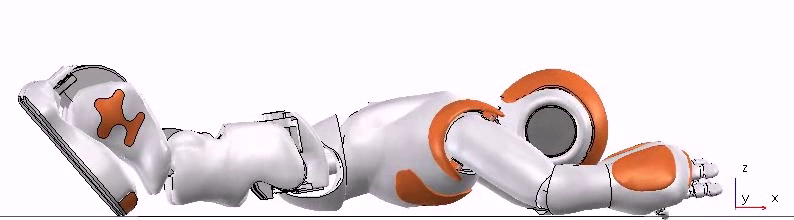
\includegraphics[width=\textwidth]{crawl/vrep/nominal/1.png}
  \caption{This figure shows the Nao humanoid V-REP simulation. 
           The robot is positioned at the initial configuration of the close chain phase
           of the crawl gait.}
  \label{fig:vrep_nao_nom_gait_single_frame1}
\end{figure}

\begin{figure}
  \centering
  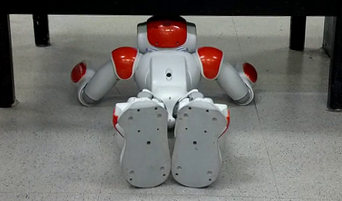
\includegraphics[height=0.35\textheight]{crawl/short_ledge1.png}
  \caption{This figure shows the Nao as it crawls under the table with the low panels.
           The head of the robot nearly touches the panel,
           representing the lowest practical traversable height constraint.}
  \label{fig:short_ledge_nao_nom_gait_single_frame1}
\end{figure}

While traversing rough terrain or over small obstacles is one application of a crawl gait,
these experiments were instead designed to show that the robot could access areas with
demanding height constraints. For this, a small table was used whose sides were blocked
with panels down to a minimum of about 200 $mm$ off of the ground. 
Figure~\ref{fig:short_ledge_nao_nom_gait_single_frame1} shows the Nao crawling under this table,
with its head almost touching the bottom of the panel. This represents the practical height
constraint that the Nao can satisfy with this gait.

% Explain that the point of this setup is to show that the crawl gait is very low profile.

\FloatBarrier
\subsection{Gait Parameters} \label{subsec:gait_params}
% Explain the gait and it's parameters.
% Nominal Parameters
As discussed in Chapter~\ref{subsec:crawl_closed_chain}, the closed chain phase of the 
Projected Profile crawl gait can be parameterized on three angles, $[\theta_3, \theta_4, \alpha]$.
These three variables are referred to as the gait parameters, or alternatively as the angle triplet.
The nominal angle triplet can be seen in Table~\ref{tab:nominal_parameters}. It holds the 
$\theta_3$ and $\theta_4$ joints constant, while increasing the angle $\alpha$ linearly as a function of time.

\begin{table}
  \centering
  \begin{tabulary}{0.5\textwidth}{|c||c|}
    \hline
    \textbf{Gait Parameter} & \textbf{Value}                \\  \hline\hline
    $\theta_3$              &   $16.5^\circ$                \\ 
    $\theta_4$              &   $27.5^\circ$                \\  
    $\alpha$                &   $-30^\circ$ to $-90^\circ$  \\  \hline
  \end{tabulary} 
  
  \caption{Table of gait parameters for the nominal crawl gait. $\theta_3$ and $\theta_4$
           are held constant, while $\alpha$ is linearly decreased in proportion to time.}
  \label{tab:nominal_parameters}
\end{table}

Results using these nominal gait parameters can be seen in Section~\ref{sec:nom_crawl_data}.

% Optimal Parameters
% PUT IN HOW MANY ITERATIONS IT TOOK TO FINISH.
% It took like 50 to 80 generations.
% PUT IN HOW MANY ITERATIONS IT TOOK TO KINDA CONVERGE.
% After 10 generations though it was already really close. 

In order to optimize the gait using these parameters, the procedure outlined in
Chapter~\ref{sec:crawl_optimization} was used, modeling the gait parameters as cubic splines.
The Genetic Algorithm in MATLAB's Global Optimization Toolbox was used in conjunction
with the V-REP torque table detailed in Chapter~\ref{subsec:crawl_pseudo_static_model}
to generate the optimal spline parameters. 
As the genetic algorithm cannot guarantee finding the global optima for any arbitrary function,
the optimization was executed several times and the best spline parameters were used
for the experiment. Each optimization used 50 to 80 generations to converge on results,
but as can be seen in Figure~\ref{fig:ga_generations}, after about 10 generations the
optimization had already reached minima and was simply exploring nearby states for possible
improvements.

\begin{figure}
  \centering
  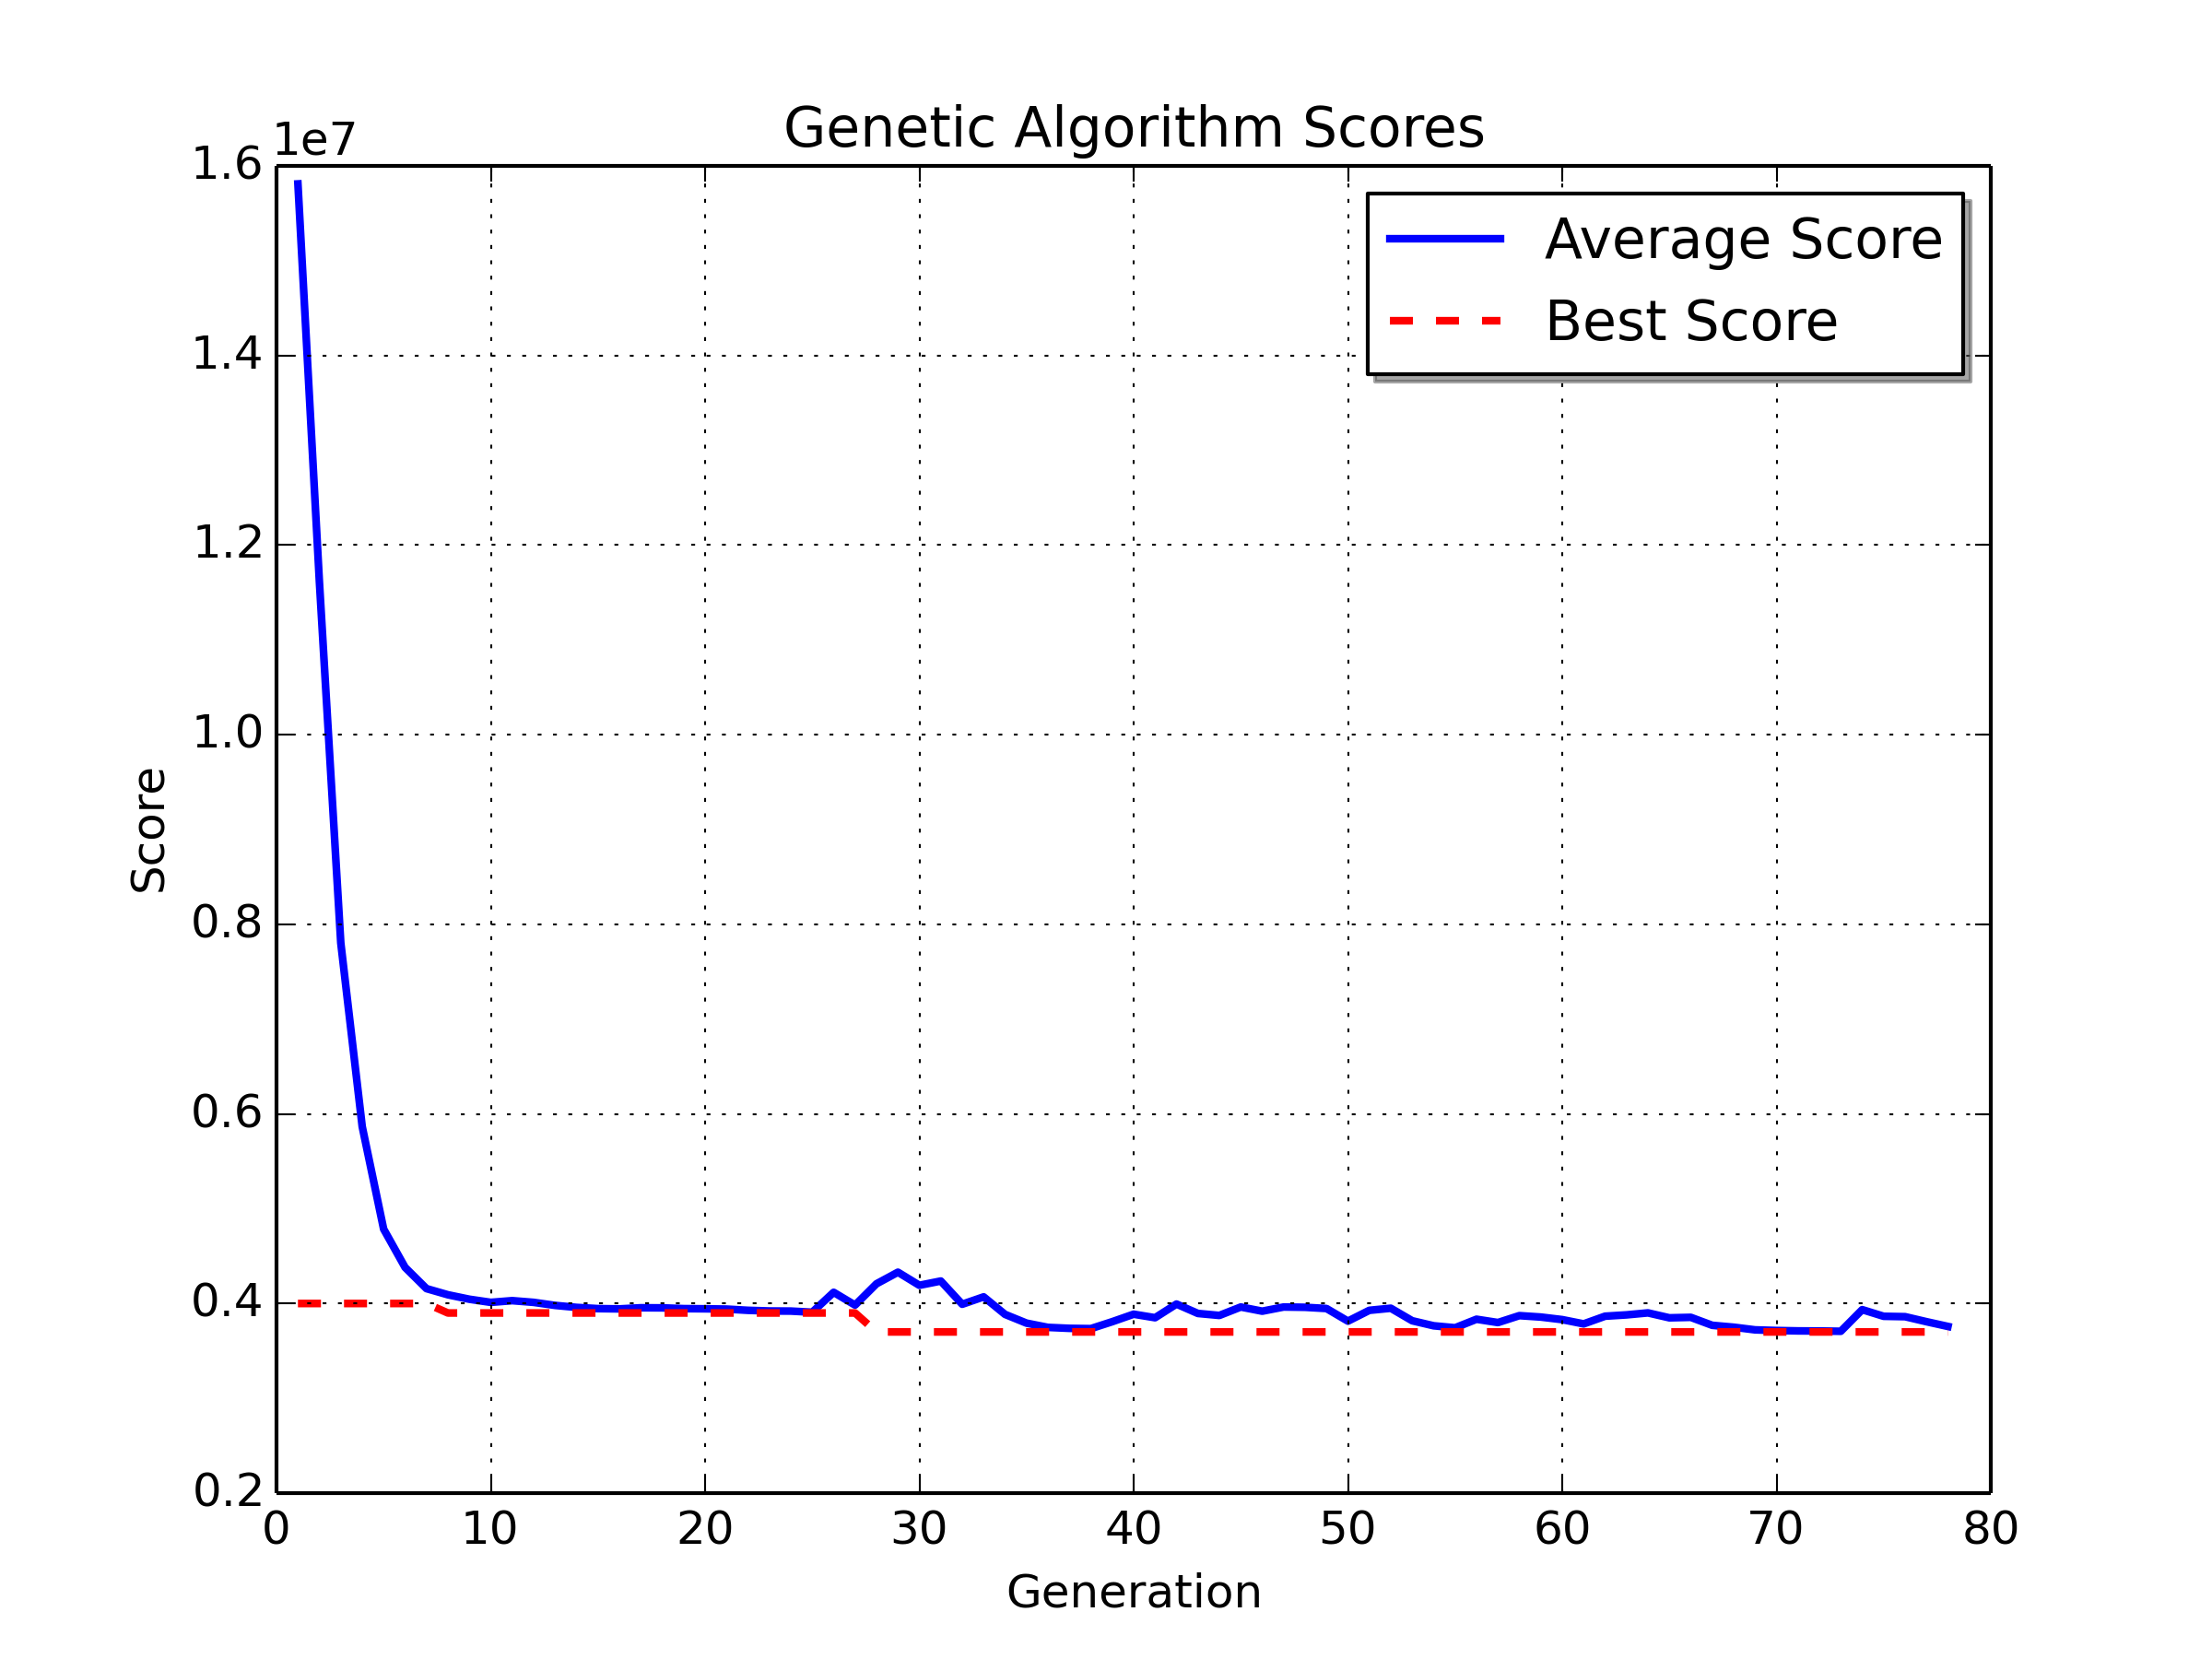
\includegraphics[height=0.35\textheight]{crawl/cost/genetic_alg_scores.png}
  \caption{This figure shows one of the gait parameter optimization trials.
           As the genetic optimization procedure uses multiple children as detailed in Chapter~\ref{subsec:crawl_opt_procedure}, the 
           plot shows the average score for the children and the score of the best
           child as the generations progress.}
  \label{fig:ga_generations}
\end{figure}

%%% TABULATE THIS
% specified initial and final values of (\alpha, \theta_3, \theta_4)
% x_init = [-30*pi/180 ; 0.28798  ;   0.47997];

% best x value found after a few runs of the genetic algorithm
% x_best = [-0.2134    1.1570   -1.9898    0.2365    0.0893   -0.3267    1.8796   -0.1365   -1.7434];

% optimized trajectory
% \alpha =   x1_ = x_best(1)*t.^3 + x_best(2)*t.^2 + x_best(3)*t + x_init(1);
% \theta_3 = x2_ = x_best(4)*t.^3 + x_best(5)*t.^2 + x_best(6)*t + x_init(2);
% \theta_4 = x3_ = x_best(7)*t.^3 + x_best(8)*t.^2 + x_best(9)*t + x_init(3);
%%%

Table~\ref{tab:optimal_parameters} shows the spine parameters resulting from the
optimization procedure. 
Each gait parameter is now a cubic polynomial which is a function of time 
$[\theta_3 (t), \theta_4 (t), \alpha (t)]$.
The coefficients from the table are used in the cubic spline $c_3 t^3 + c_2 t^2 + c_1 t + c_0$.
The gait parameter splines are constrained by the starting and ending angles for each parameter.
When $t = 0$, the splines must produce the starting angles for the triplet, 
$[\theta_3 (0), \theta_4 (0), \alpha (0)] = [0.28798, 0.47997, 0.52360]$.
At the final time $t = t_f$, the splines must produce 
$[\theta_3 (t_f), \theta_4 (t_f), \alpha (t_f)] = [0.28798, 0.47997, -1.5710]$. 
The initial and final angle triplets are in radians.

\begin{table}
  \centering
  \begin{tabulary}{0.75\textwidth}{|c|c|c|c|c|}
    \hline
    \textbf{Gait Parameter} & \textbf{$c_3$} & \textbf{$c_2$} & \textbf{$c_1$} & \textbf{$c_0$} \\  \hline\hline
    $\theta_3$              &   0.2365       &  0.0893        & -0.3267        &  0.28798       \\ 
    $\theta_4$              &   1.8796       & -0.1365        & -1.7434        &  0.47997       \\  
    $\alpha$                &  -0.2134       &  1.1570        & -1.9898        &  0.52360       \\  \hline
  \end{tabulary} 
  
  \caption{Table of gait parameter coefficients for the optimal crawl gait. 
           The $c_i$ coefficients are used in the cubic spline 
           $c_3 t^3 + c_2 t^2 + c_1 t + c_0$ to vary the gait parameters as a function of time.
           The $c_0$ coefficients are simply the initial starting angles for each parameter.}
  \label{tab:optimal_parameters}
\end{table}

Figure~\ref{fig:optimal_gait_parameters} shows the splines graphically, with the nominal gait parameters
overlaid for comparison. While the optimized parameter trajectory for $\alpha$ is similar to its nominal
trajectory, the trajectories for $\theta_3$ and $\theta_4$ dip significantly, with $\theta_4$ having the
most drastic deviation from the nominal.

\begin{figure}
\centering
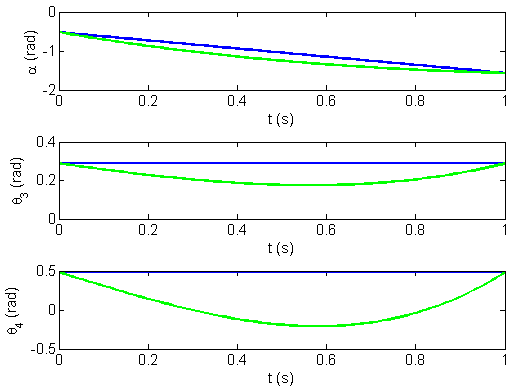
\includegraphics[width=0.75\textwidth]{crawl/cost/ga_cost2_plot1_edit1.png}  
\caption{This figure shows the optimal gait parameter trajectories overlaid onto the nominal
         trajectories. The blue lines represent the nominal trajectories while the green
         lines show the optimal.}
\label{fig:optimal_gait_parameters}
\end{figure}




\FloatBarrier
\section{Nominal Crawl Gait Data} \label{sec:nom_crawl_data}

% As reviewed in Section \ref{subsec:gait_params}, ...
% This experiment was done using nominal parameters.
% This is basic thing to do.
To test the Projected Profile gait using the nominal parameters reviewed in 
Section~\ref{subsec:gait_params}, the gait sequence was first generated in
MATLAB and then simulated in V-REP\@. Following this, the gait was tested on the
Nao by setting it to crawl under a vertically constrained table in two different
experiments. In the first, the robot was set to the initial crawling pose and
placed on the floor in front of the table. The robot then executed the crawling gait.
In the second experiment the robot was programmed to recognize a fiducial marker,
represented by a red circle mounted to the table, and walk to it. 
The robot then moved to a prone posture and crawled under the table. This procedure
is more throughly examined in Section~\ref{sec:crawl_exp_setup}. Joint angle and joint
motor current data was collected during the table experiments and is presented in this section.
These table experiments demonstrate the efficacy of the gait to locomote the robot
and the low profile nature of the gait to allow access to vertically constrained spaces.

\subsection{Simulations}
% Here's the MATLAB Projected Profile gait. You can see it moves the mass forward.
% You can see the theta 3 and 4 are held static.
Figure~\ref{fig:pp_nom_gait1} shows samples of the closed chain phase of the Projected
Profile gait using the nominal parameters. It shows a simplified kinematic model
representing a projection of the robot onto the saggital plane. The frames show the
model starting in the initial pose, and by linearly increasing the $\alpha$ gait
parameter and holding the $\theta_3$ and $\theta_4$ parameters constant, the model
shifts forward until $\alpha$ has reached its terminal value of $-90^\circ$. This places the model
at the final closed chain pose. It can be seen that the highest point of this gait occurs
when the ankle joint is at about $z =$ 100 $mm$. This model of course does not include the limb thicknesses nor
the head of the Nao, as it only models joint centers. This model was created using MATLAB
and is used to view the results of the gait sequence generation.

\begin{figure}
\centering
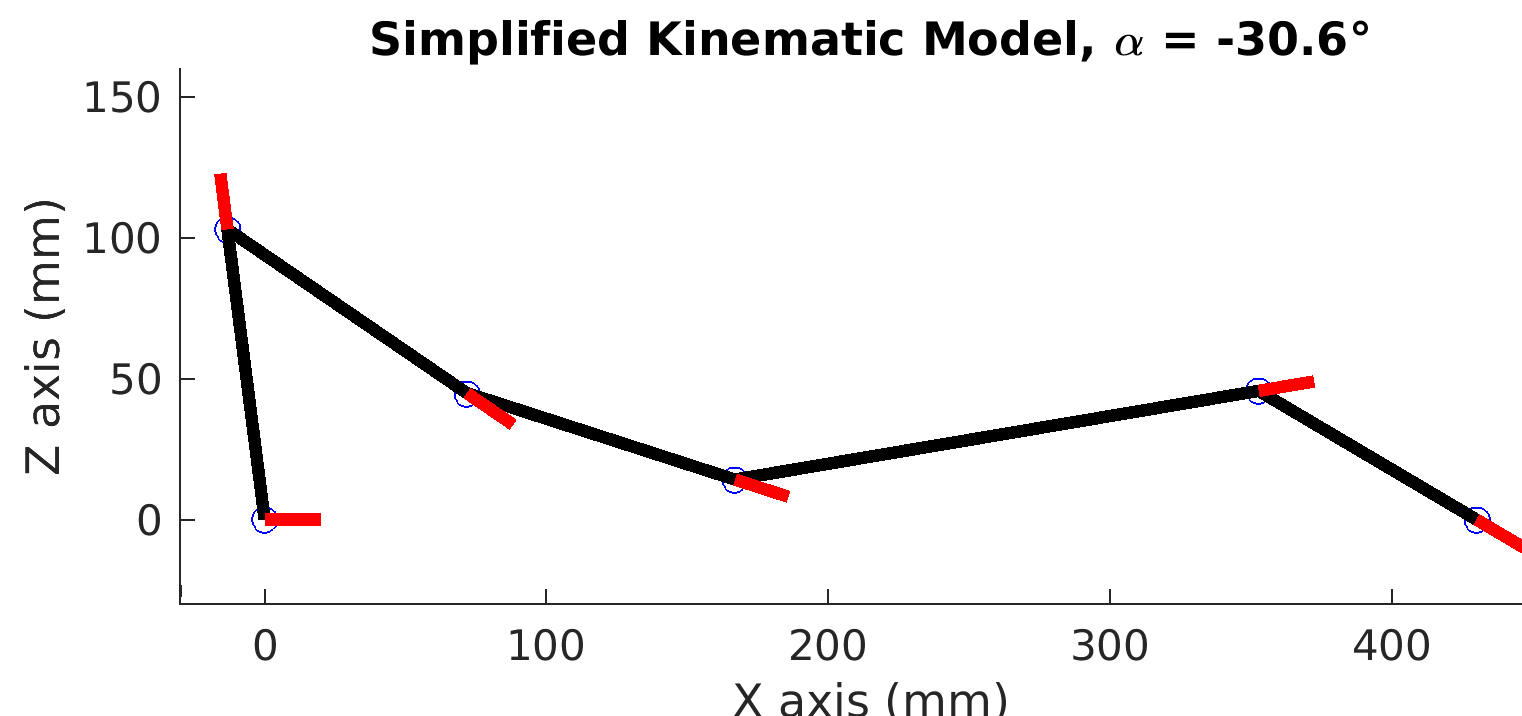
\includegraphics[width=0.5\textwidth]{crawl/pp/nominal/angle30.6_1.png}
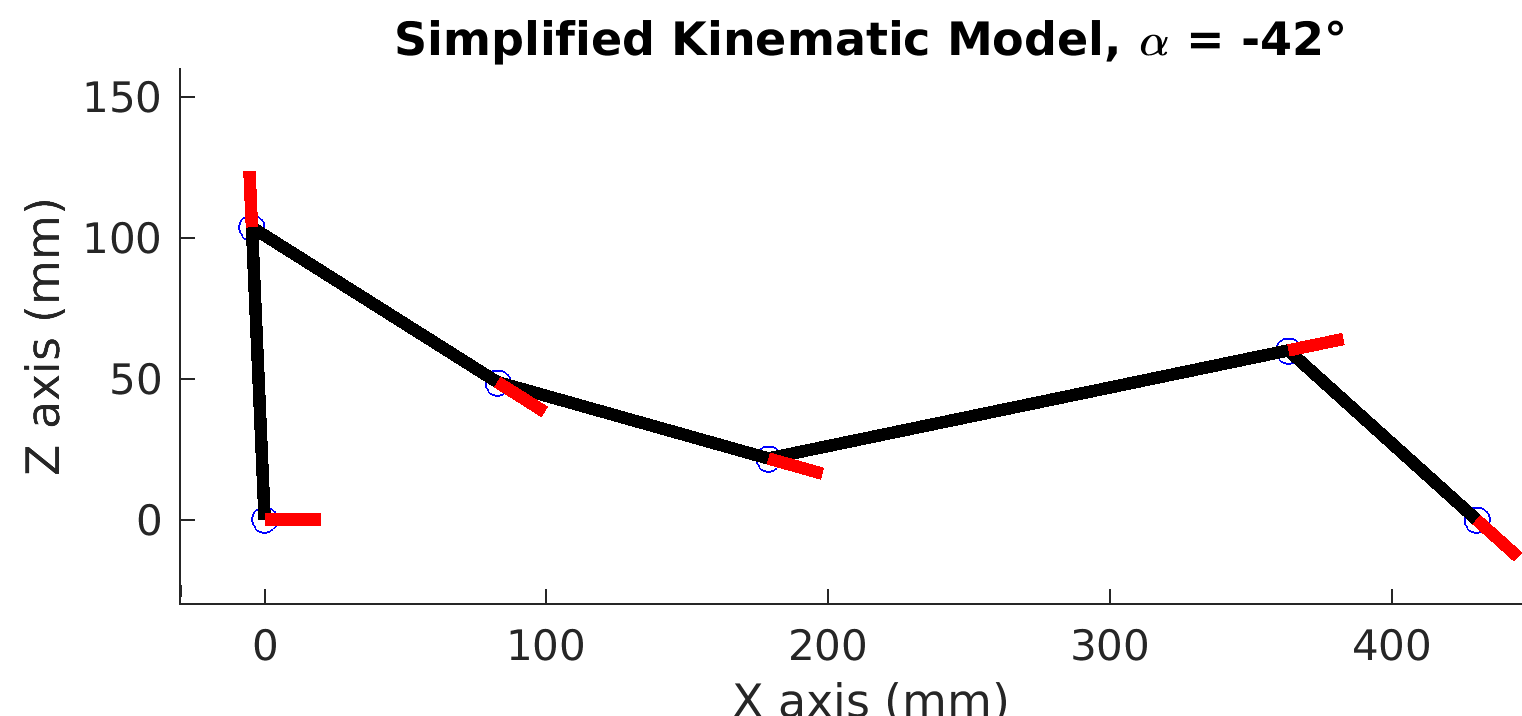
\includegraphics[width=0.5\textwidth]{crawl/pp/nominal/angle42_1.png}
\centering
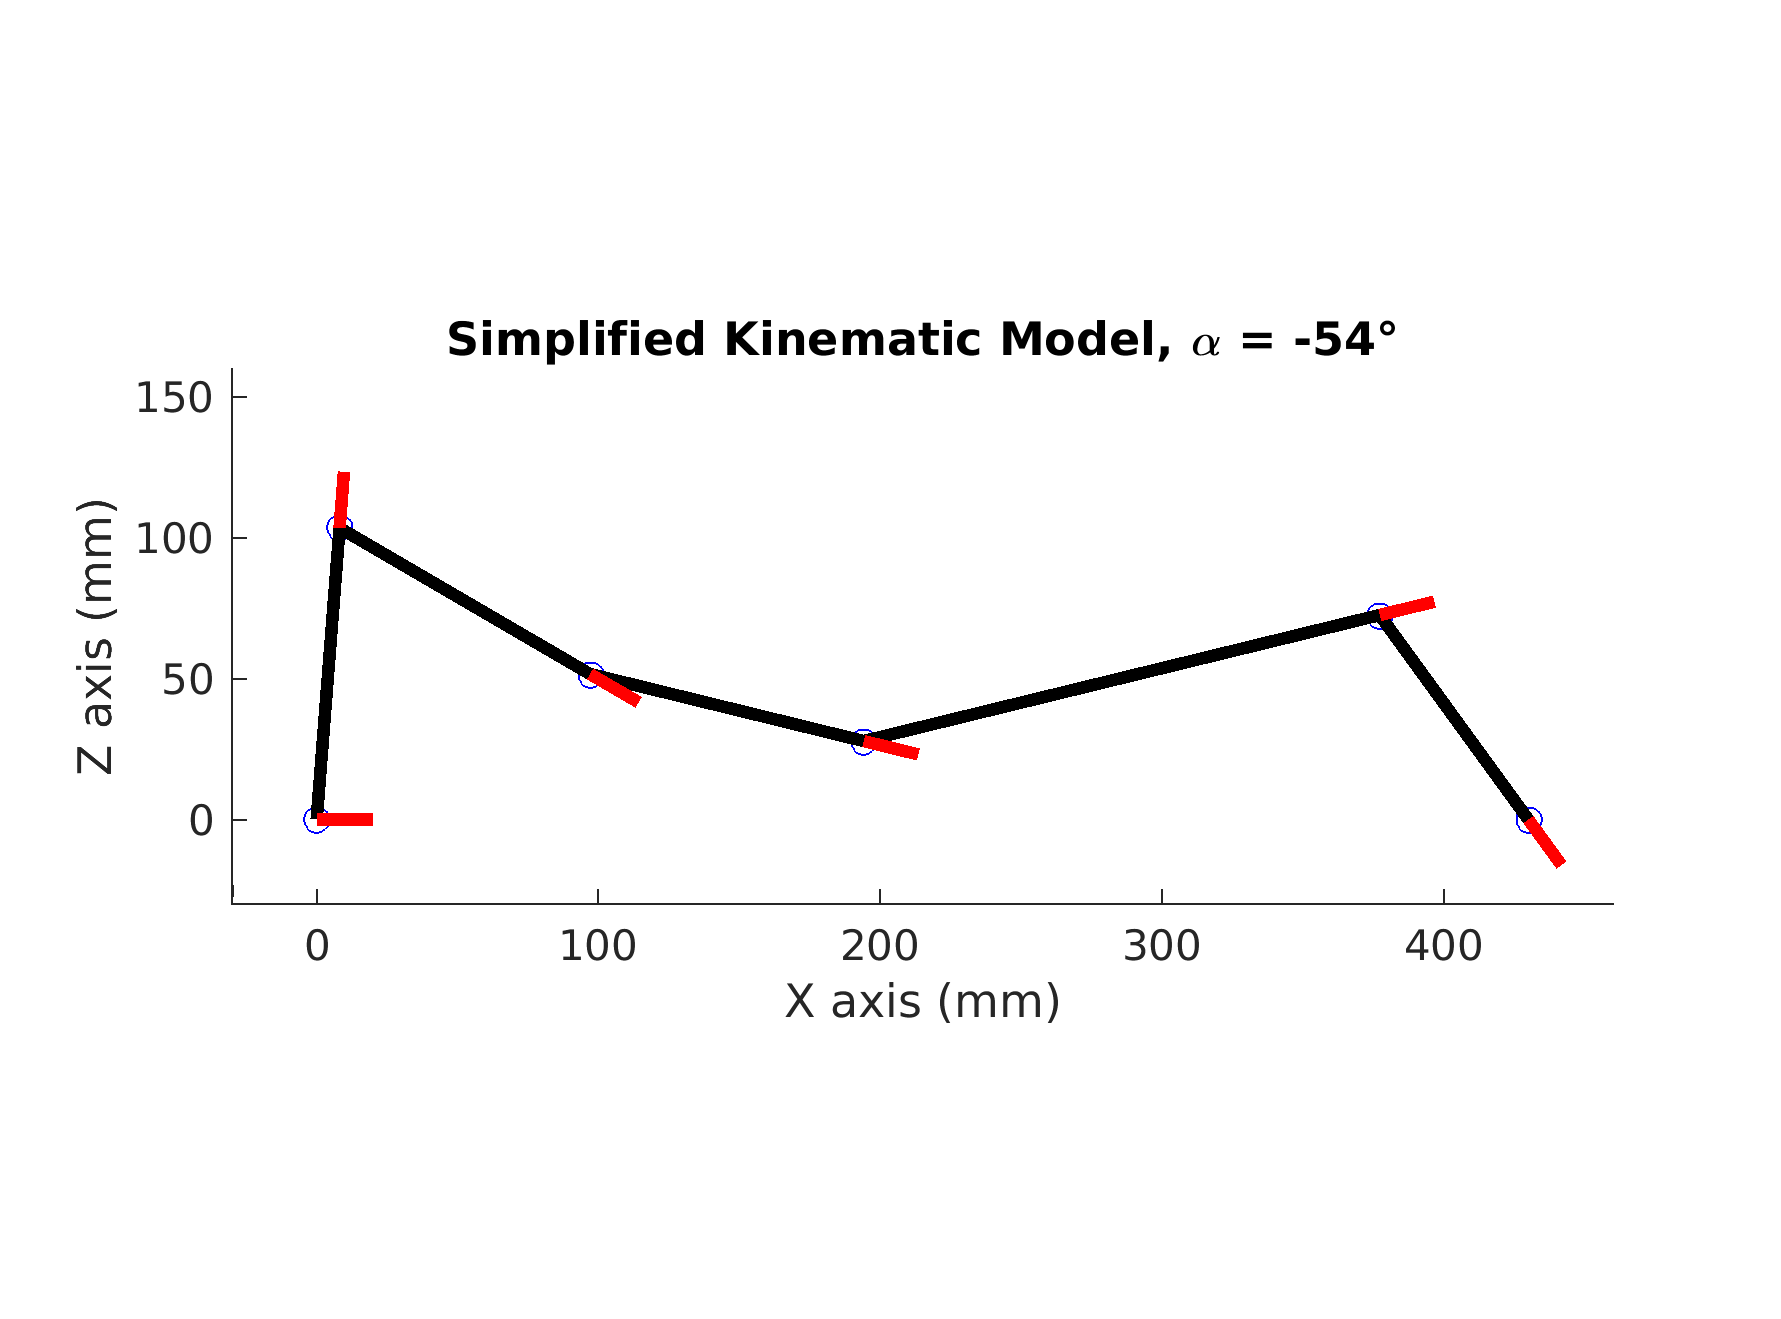
\includegraphics[width=0.5\textwidth]{crawl/pp/nominal/angle54_1.png}
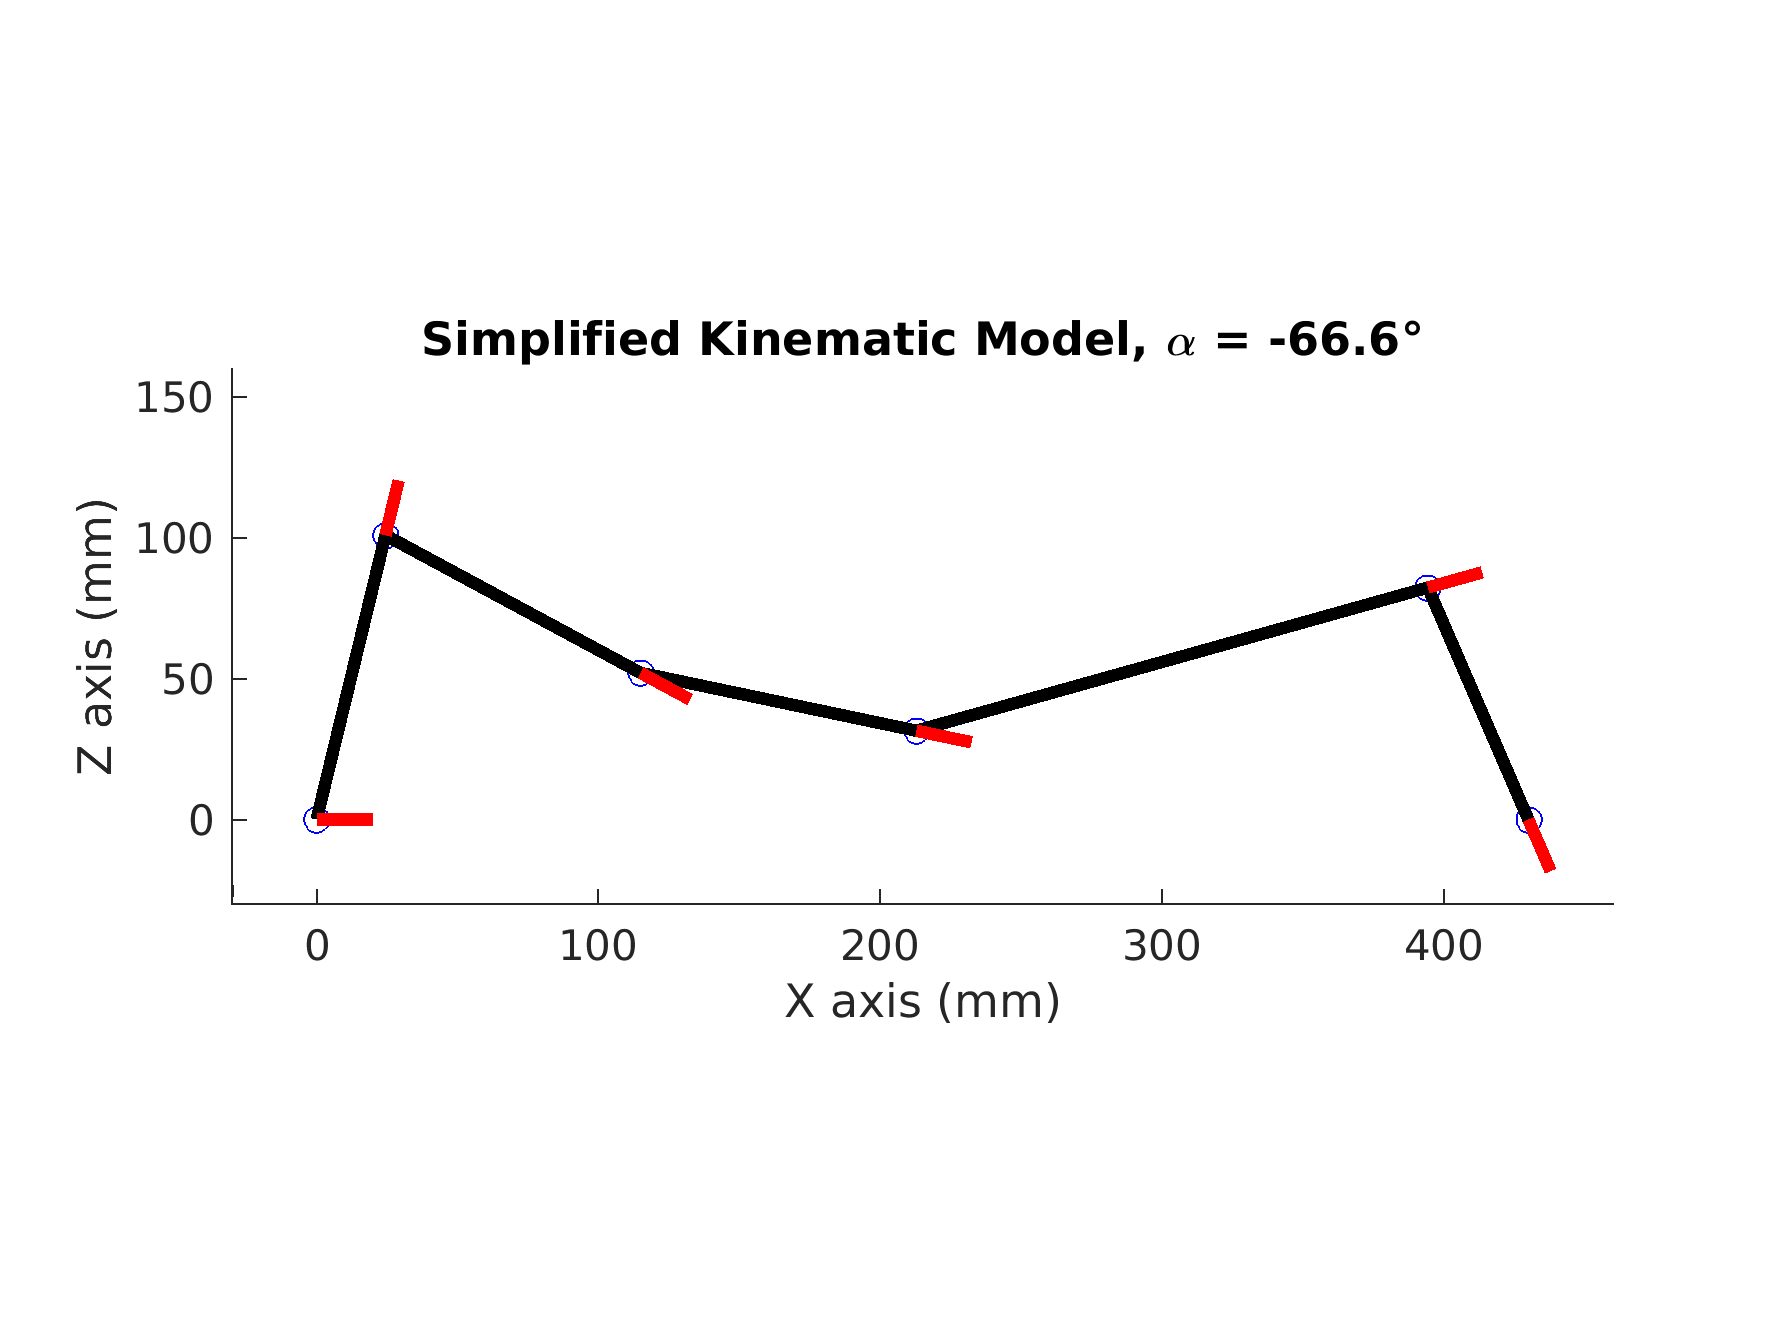
\includegraphics[width=0.5\textwidth]{crawl/pp/nominal/angle66.6_1.png}
\centering
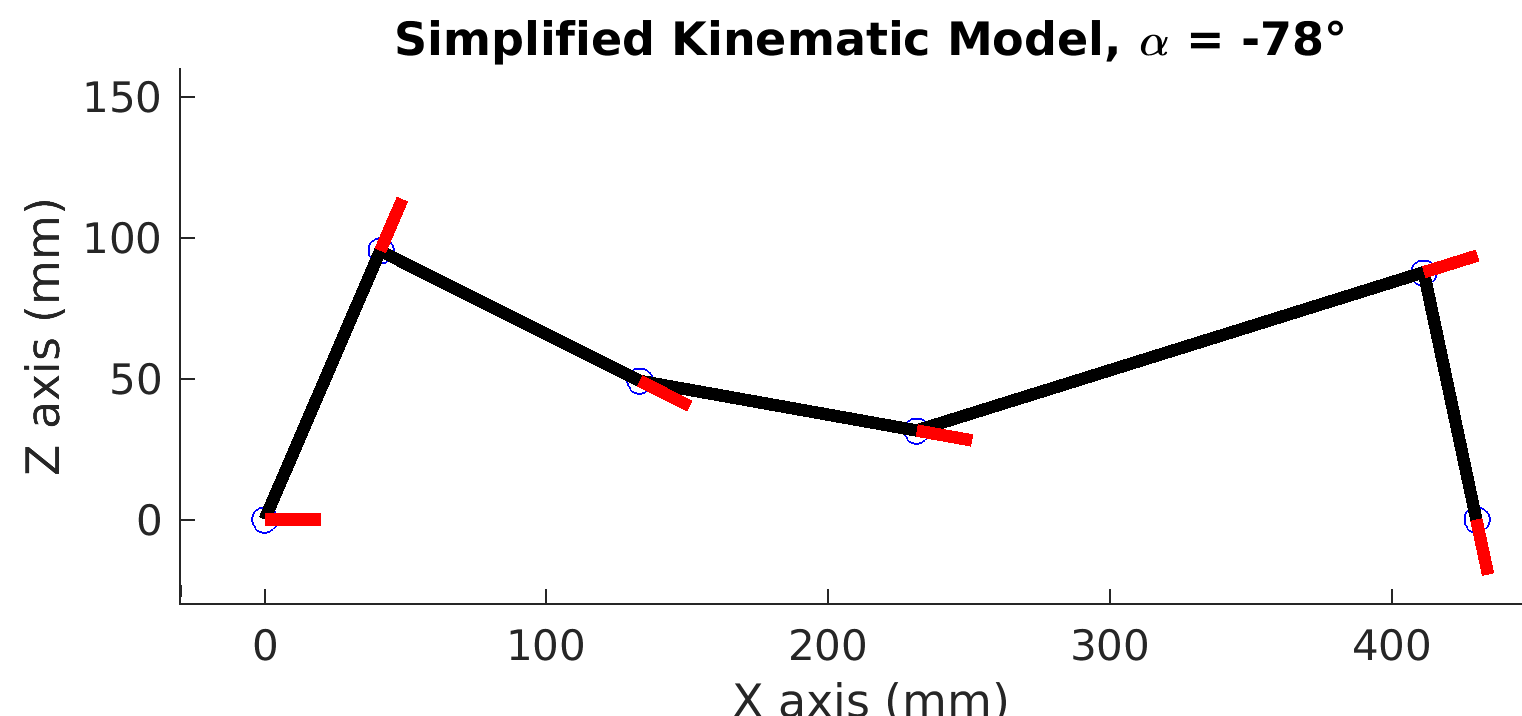
\includegraphics[width=0.5\textwidth]{crawl/pp/nominal/angle78_1.png}
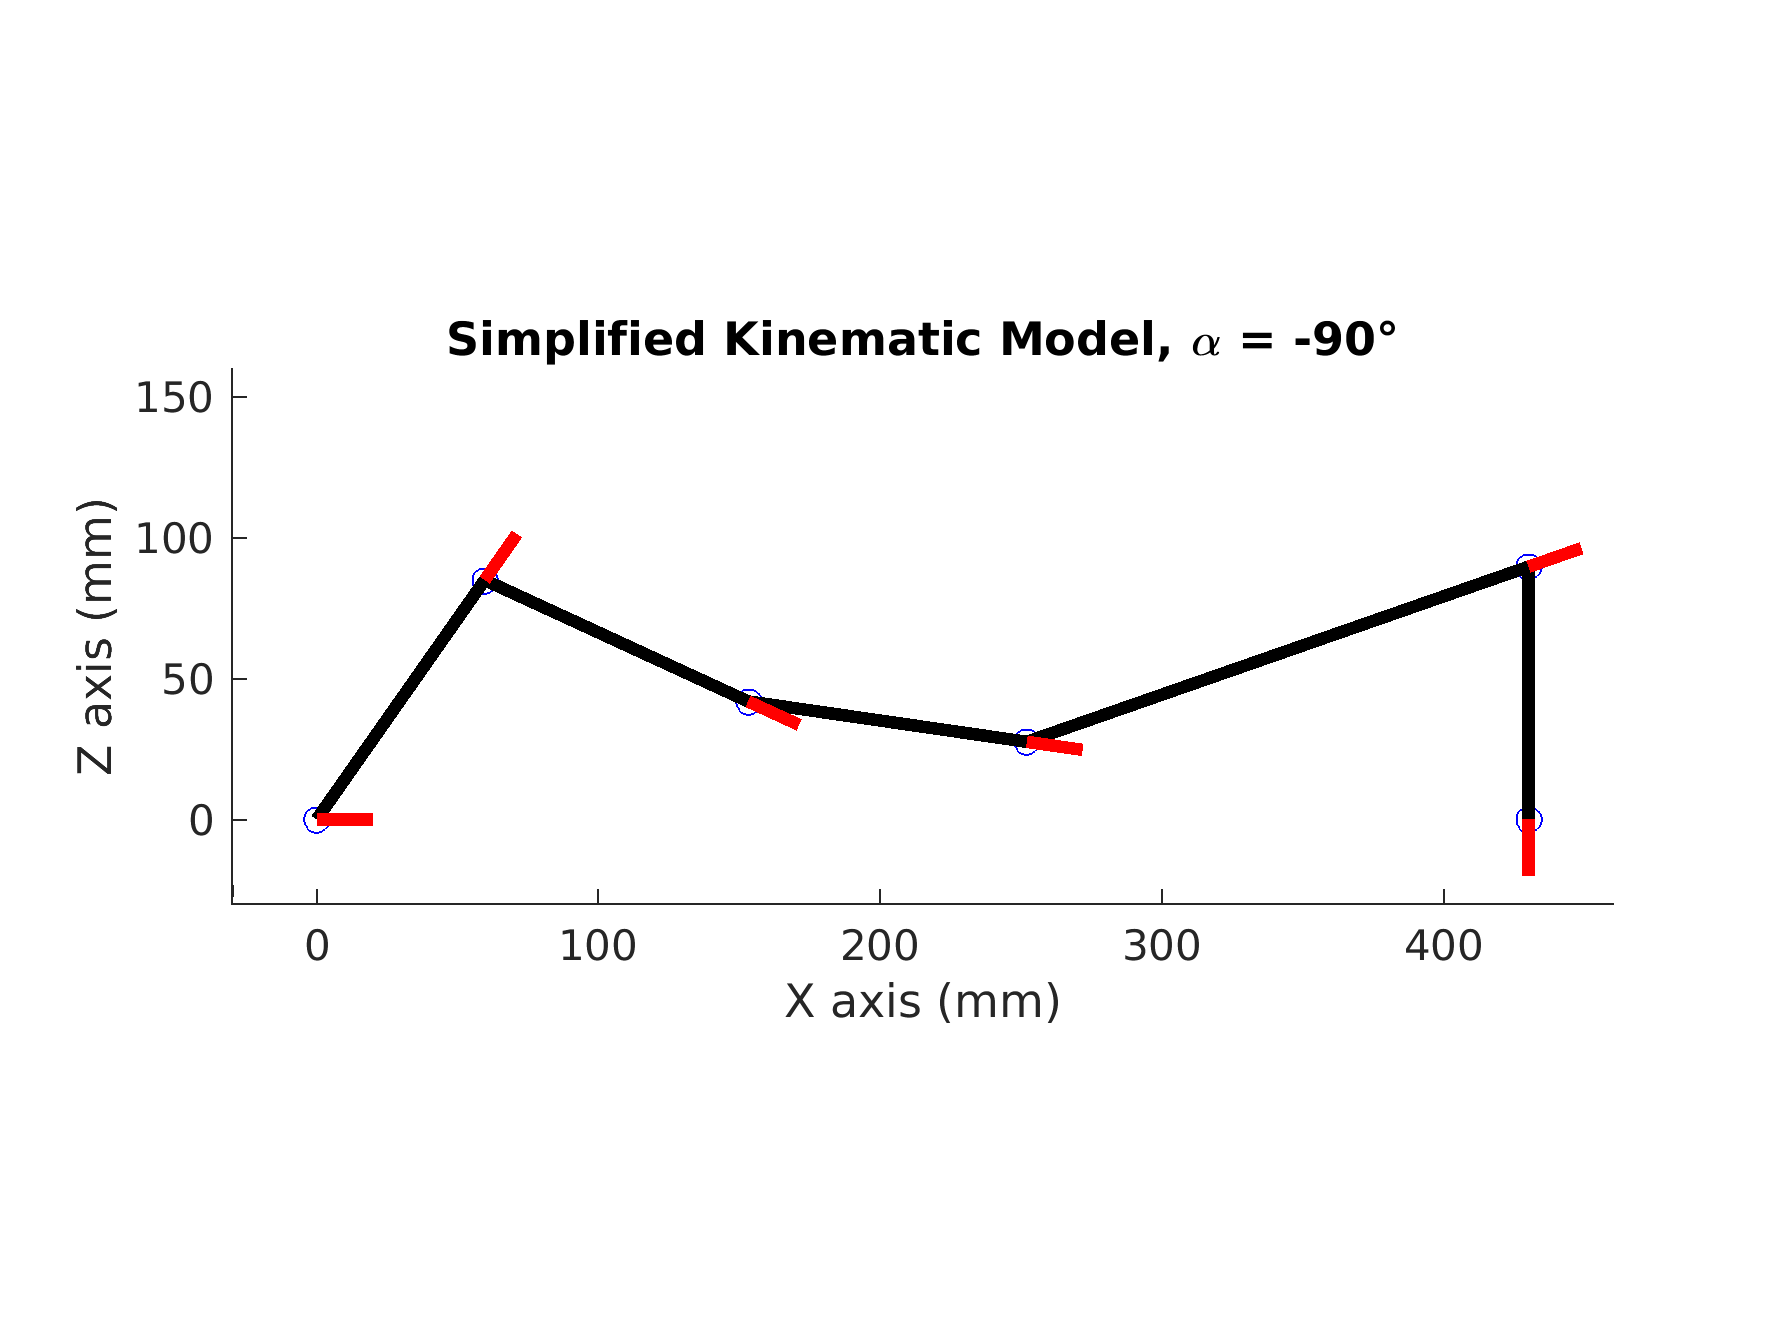
\includegraphics[width=0.5\textwidth]{crawl/pp/nominal/angle90_1.png}
\caption{This figure shows a simplified kinematic model of the Nao as it executes
         the Projected Profile gait using nominal parameters. The model starts with
         $\alpha = -30^\circ$ and terminates when $\alpha = -90^\circ$.}
\label{fig:pp_nom_gait1}
\end{figure}

% Here's the V-REP gait. You can see it moves the mass forward.
% The arms are down the whole time.
% You can see the knee and hip are held static.

Once the gait sequence is generated, it is tested using the V-REP simulation of the
Nao humanoid. Figure~\ref{fig:vrep_nao_nom_gait1} shows the simulated Nao executing
the closed chain phase of the nominal crawl gait. As with the simplified kinematic
model, the $\alpha$ gait parameter is linearly increased from $-30^\circ$ to $-90^\circ$,
which moves the robot forward. As detailed in Chapter~\ref{subsec:nao_kinematics}, the
gait parameters and other constraints are used to position the arms of the robot. Unlike
the ankle pitch, hip pitch, and shoulder pitch joints which have angles that directly correspond to
joint angles in the simplified kinematic model, the shoulder roll, elbow yaw, and elbow roll joints
do not. The head in this simulation can be seen to be the highest part of the robot
throughout the majority of the gait, increasing the minimum value of the allowable
vertical constraint.

\begin{figure}
\centering
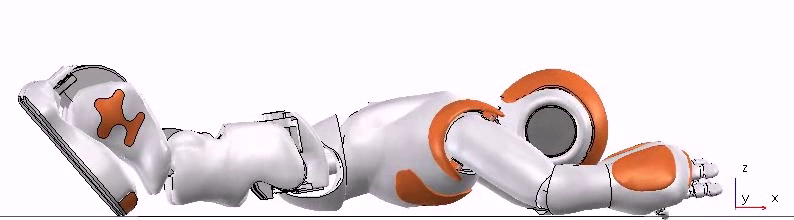
\includegraphics[width=0.5\textwidth]{crawl/vrep/nominal/1.png}
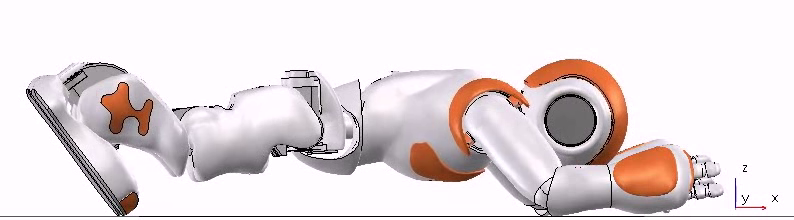
\includegraphics[width=0.5\textwidth]{crawl/vrep/nominal/2.png}
  
\centering
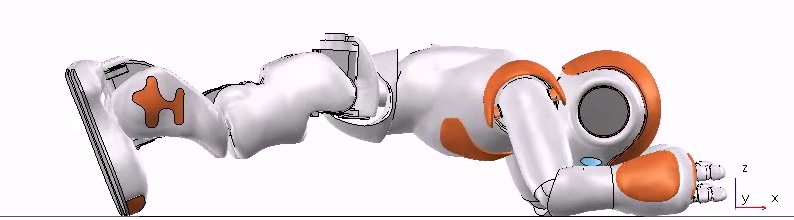
\includegraphics[width=0.5\textwidth]{crawl/vrep/nominal/3.png}
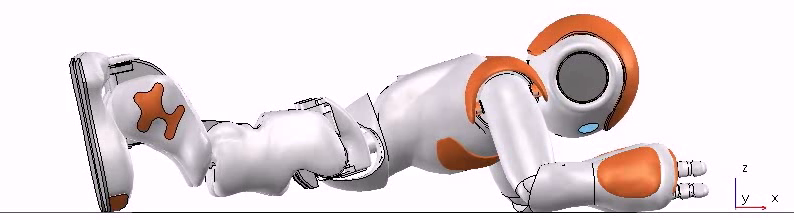
\includegraphics[width=0.5\textwidth]{crawl/vrep/nominal/4.png}
  
\centering
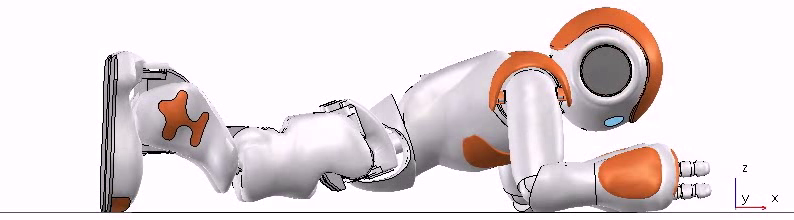
\includegraphics[width=0.5\textwidth]{crawl/vrep/nominal/5.png}

\caption{This figure shows the simulated Nao executing the closed chain phase
         of the gait using the nominal parameters.}
\label{fig:vrep_nao_nom_gait1}
\end{figure}

\subsection{Vertically Constrained Table}

% Here's the Nao doing the crawl under a little ledge.
% You can see it's really low profile.

Following simulation, the Projected Profile crawl gait using the nominal parameters
was tested on the Nao. Figure~\ref{fig:nao_table_exp1_crawl1} shows the initial test of the
robot crawling under the vertically constrained table. The Nao is set to the initial
crawling pose on the floor outside of the table. The robot then executes the crawl
gait for several sequences until the robot is under the table.
For this experiment, the robot executed 9 sequences in 27 seconds. The robot traveled
about 1 body length or 610 $mm$, equating to a velocity of 22.6 $\frac{mm}{s}$.

% \begin{figure}
%   \centerline{
%     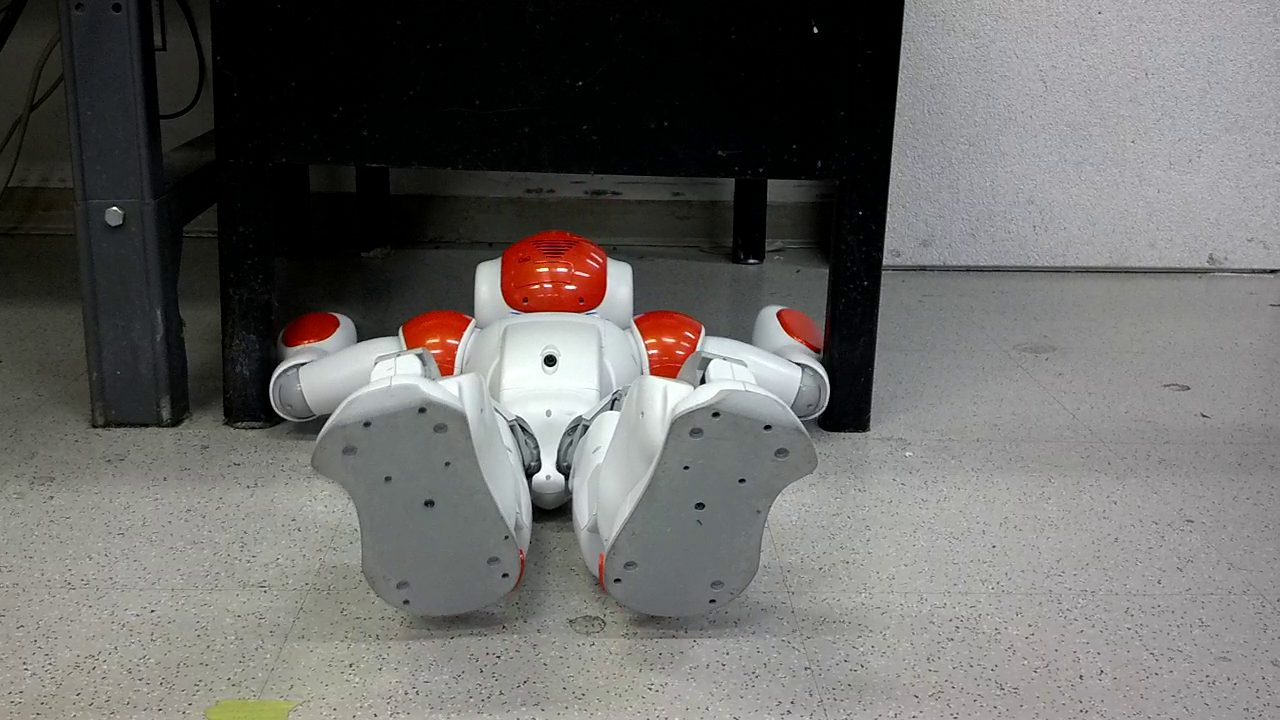
\includegraphics[width=0.25\textwidth]{crawl/under_table/14s.png}
%     \includegraphics[width=0.25\textwidth]{crawl/under_table/18s.png}
%     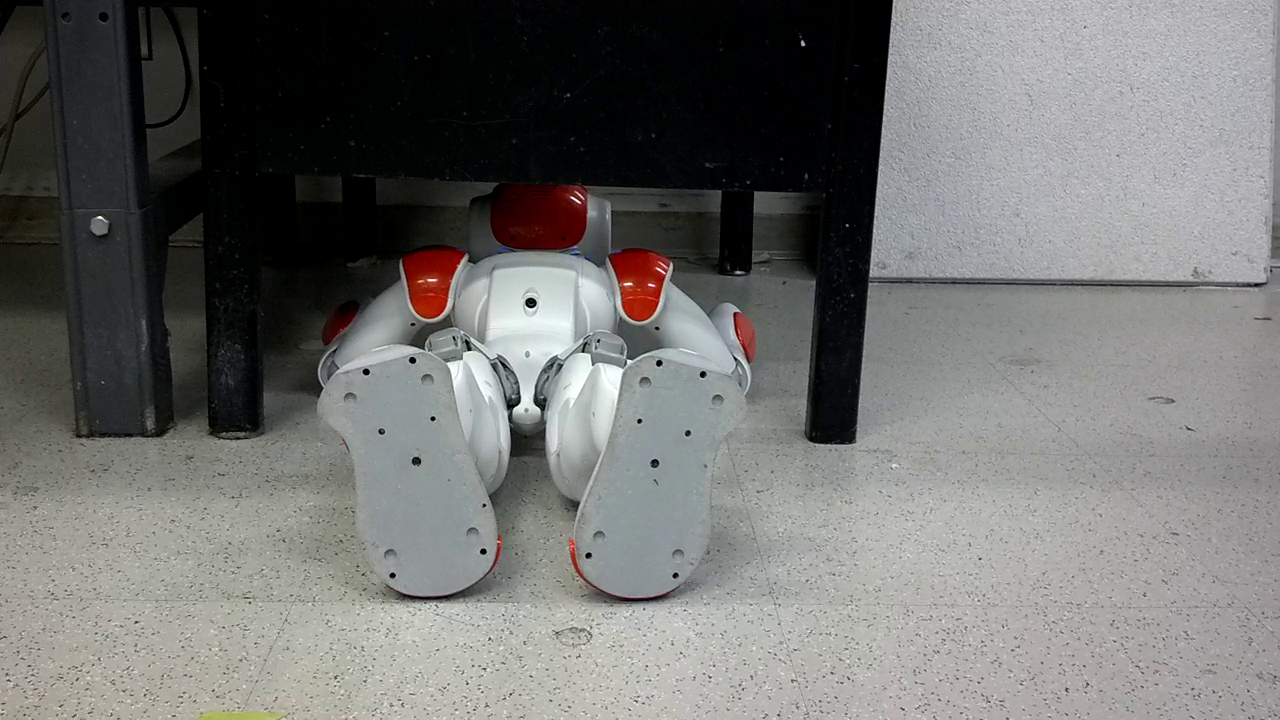
\includegraphics[width=0.25\textwidth]{crawl/under_table/19s.png}
%     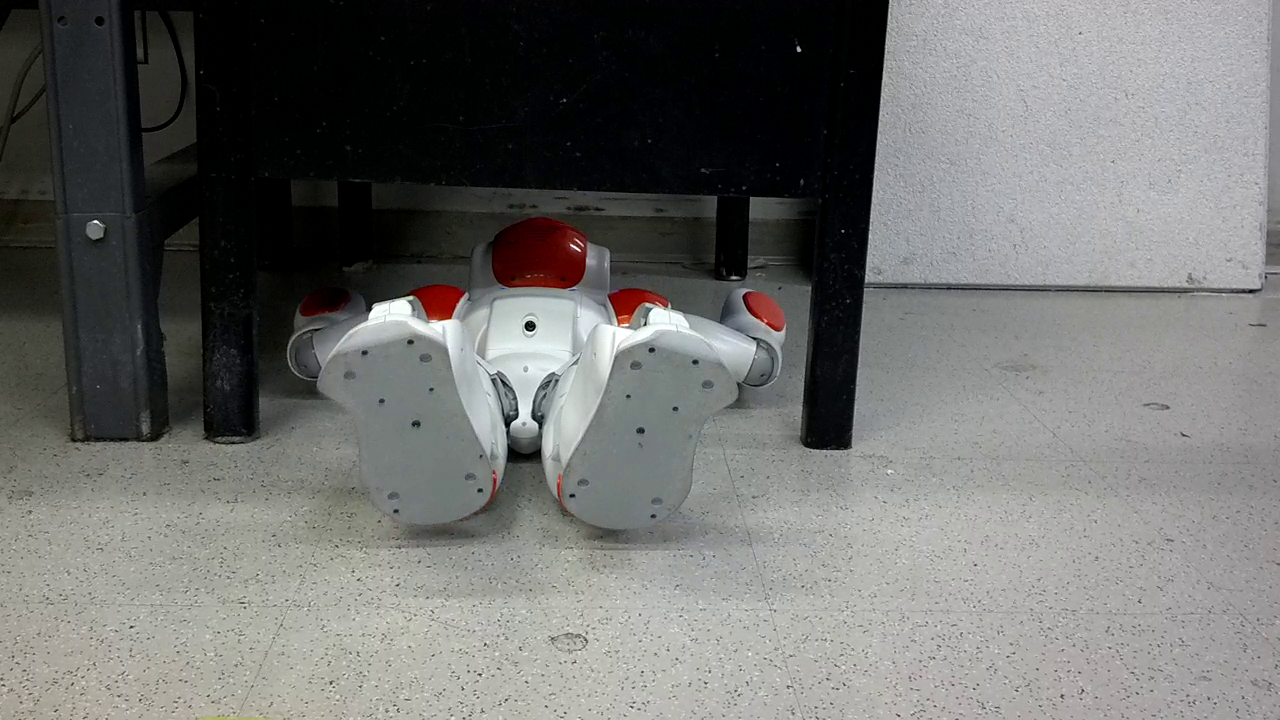
\includegraphics[width=0.25\textwidth]{crawl/under_table/20s.png}
%   }
%   \caption{Low-profile crawling gait for accessing vertically constrained spaces such as under a table.}
%   \label{fig:nao_crawl1}
% \end{figure}

\begin{figure}
\centering
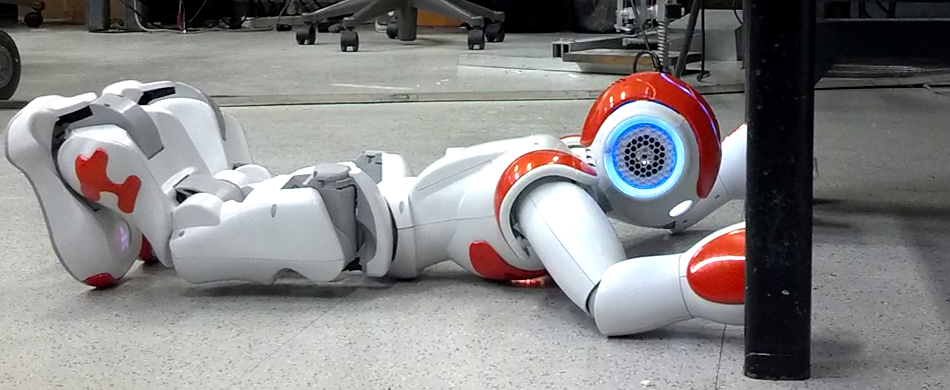
\includegraphics[width=0.33\textwidth]{crawl/under_table/profile_sequence/01.png}
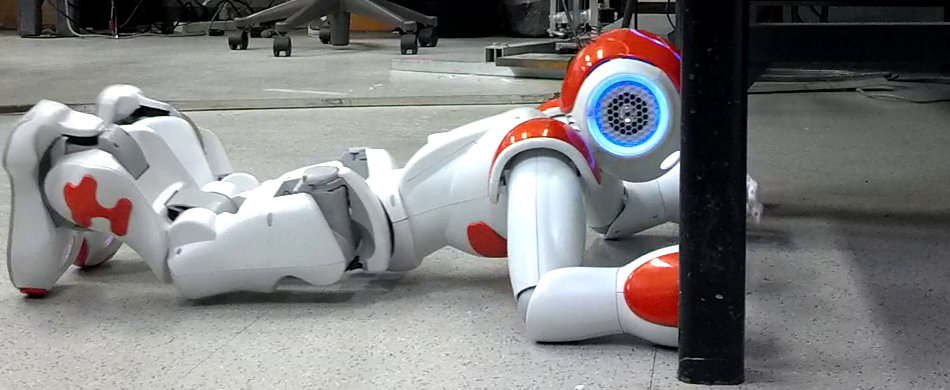
\includegraphics[width=0.33\textwidth]{crawl/under_table/profile_sequence/02.png}
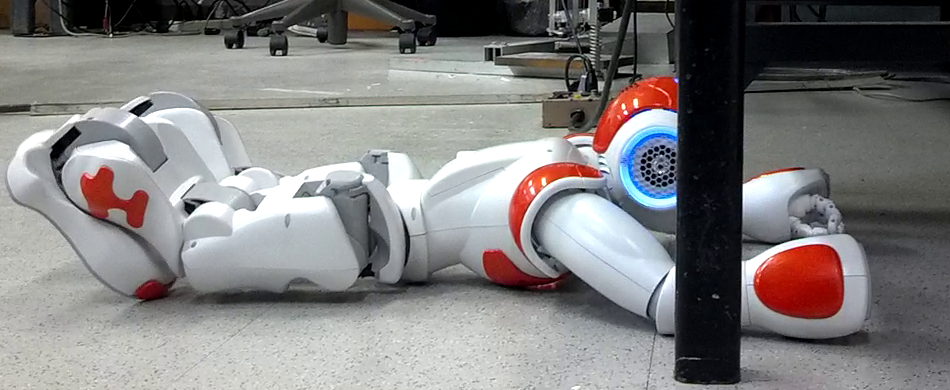
\includegraphics[width=0.33\textwidth]{crawl/under_table/profile_sequence/03.png}

\vspace*{0.05in}
\centering
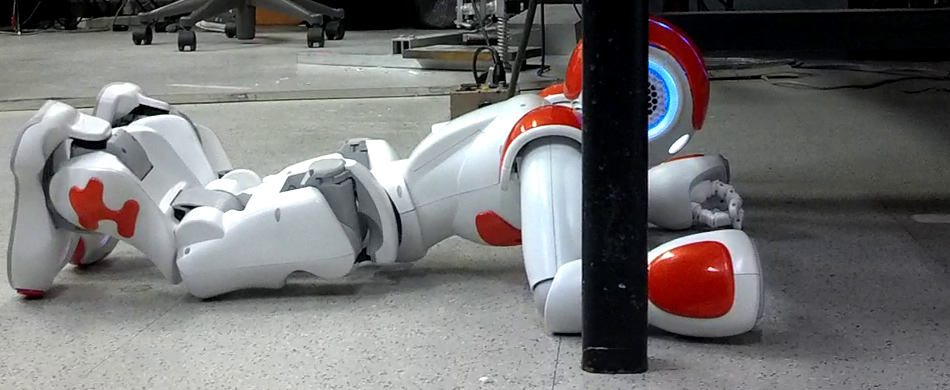
\includegraphics[width=0.33\textwidth]{crawl/under_table/profile_sequence/04.png}
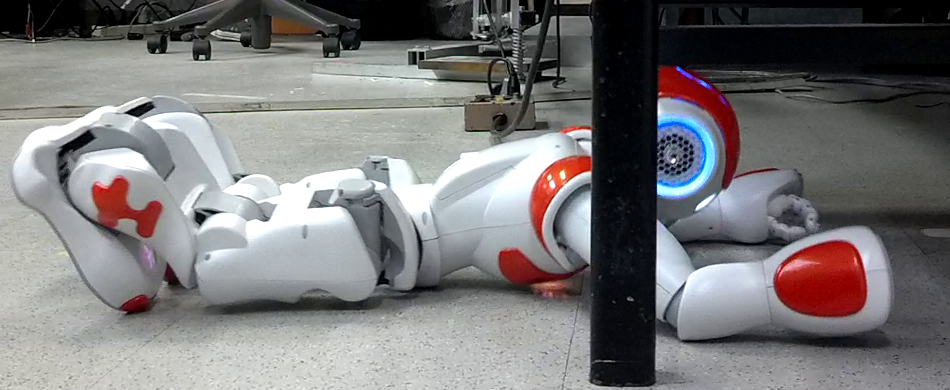
\includegraphics[width=0.33\textwidth]{crawl/under_table/profile_sequence/05.png}
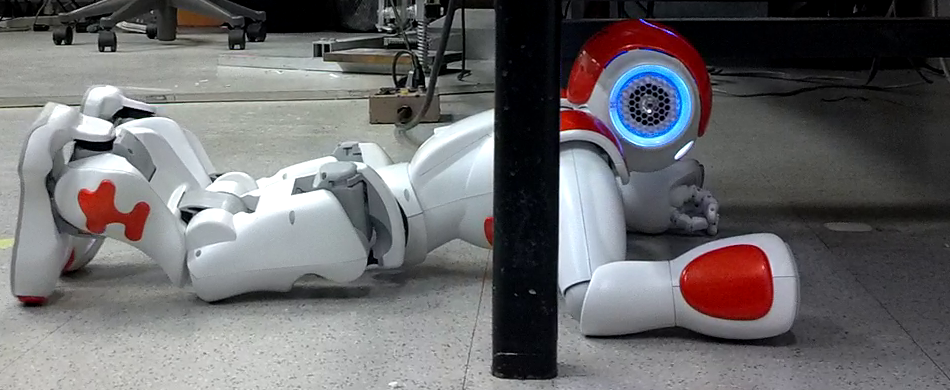
\includegraphics[width=0.33\textwidth]{crawl/under_table/profile_sequence/06.png}

\vspace*{0.05in}
\centering
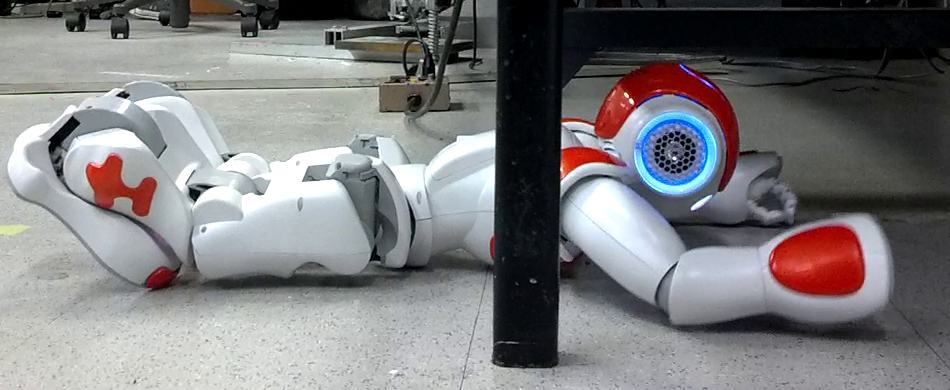
\includegraphics[width=0.33\textwidth]{crawl/under_table/profile_sequence/07.png}
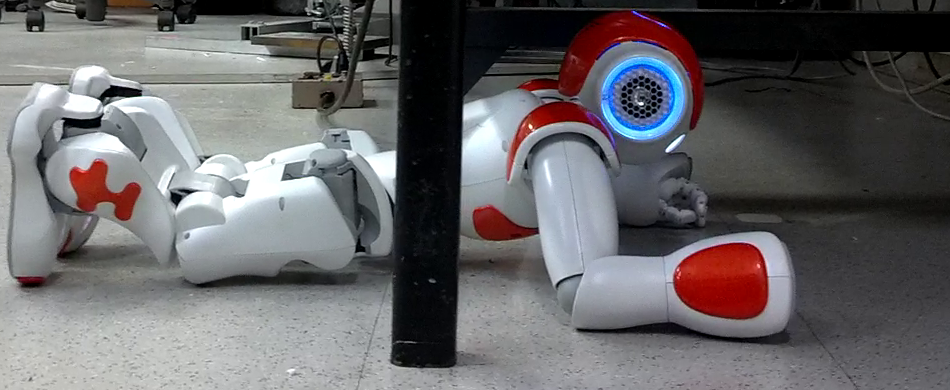
\includegraphics[width=0.33\textwidth]{crawl/under_table/profile_sequence/08.png}
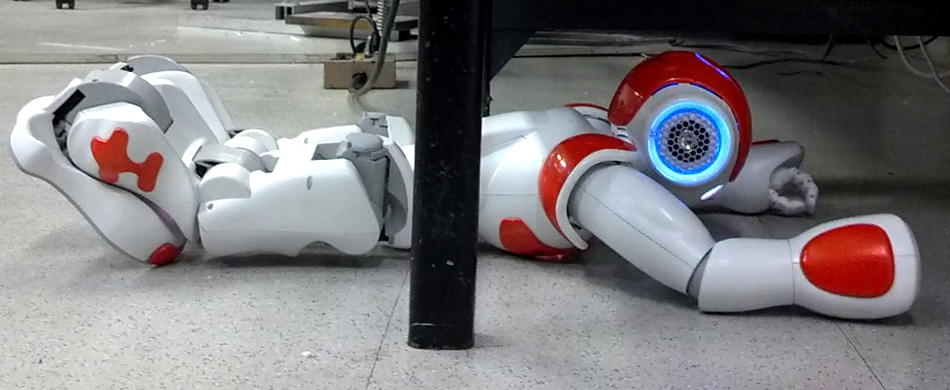
\includegraphics[width=0.33\textwidth]{crawl/under_table/profile_sequence/09.png}

\vspace*{0.05in}
\centering
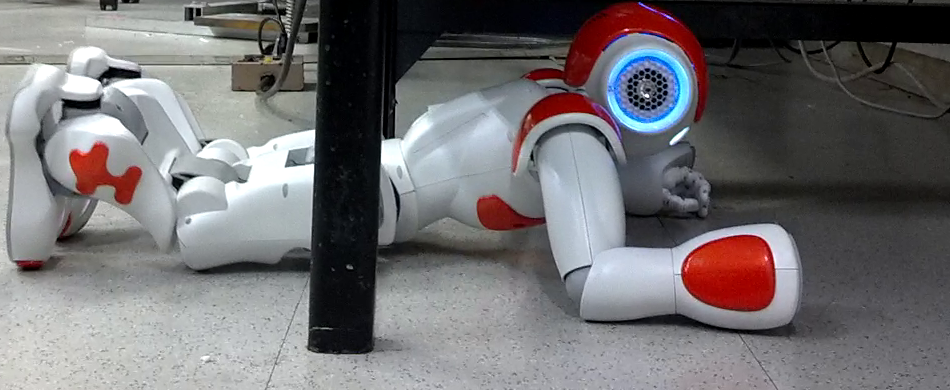
\includegraphics[width=0.33\textwidth]{crawl/under_table/profile_sequence/10.png}
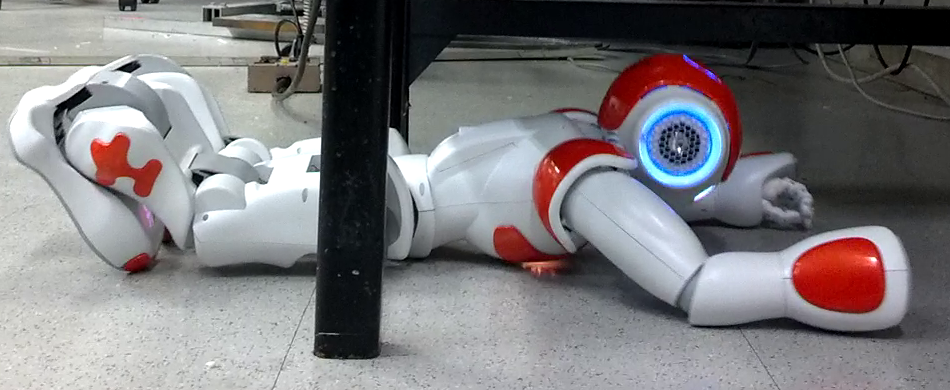
\includegraphics[width=0.33\textwidth]{crawl/under_table/profile_sequence/11.png}
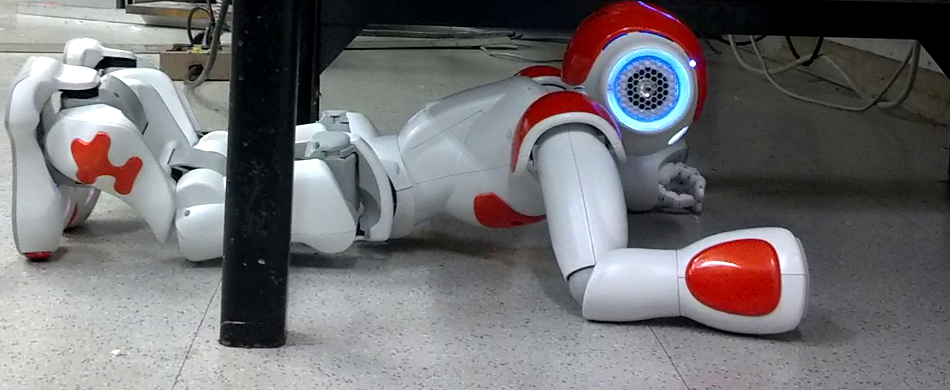
\includegraphics[width=0.33\textwidth]{crawl/under_table/profile_sequence/12.png}

\vspace*{0.05in}
\centering
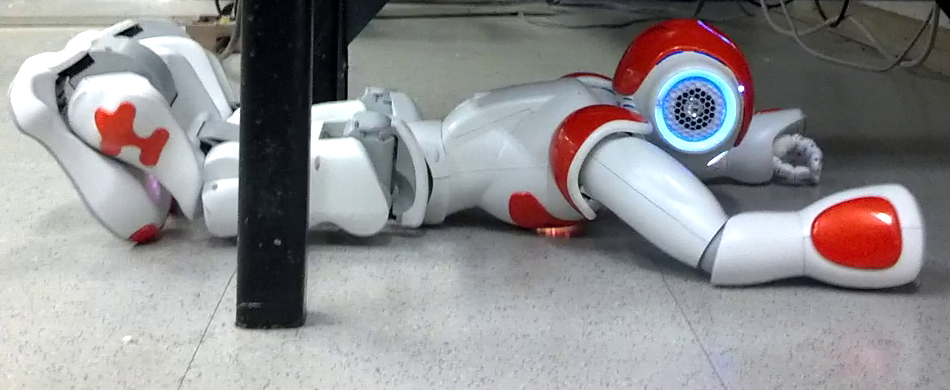
\includegraphics[width=0.33\textwidth]{crawl/under_table/profile_sequence/13.png}
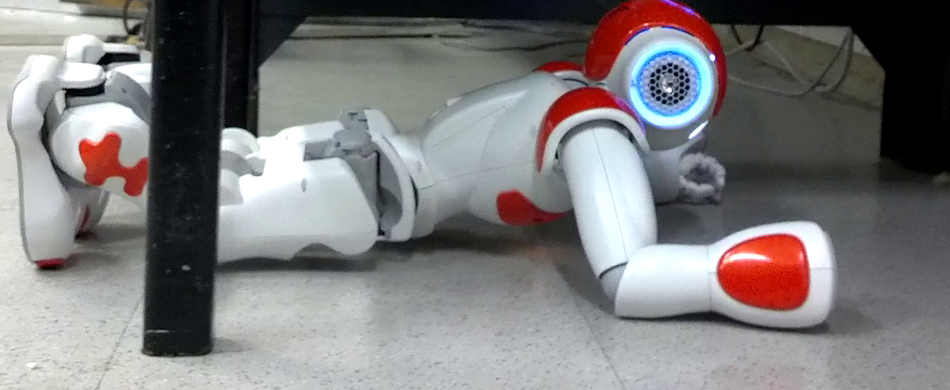
\includegraphics[width=0.33\textwidth]{crawl/under_table/profile_sequence/14.png}
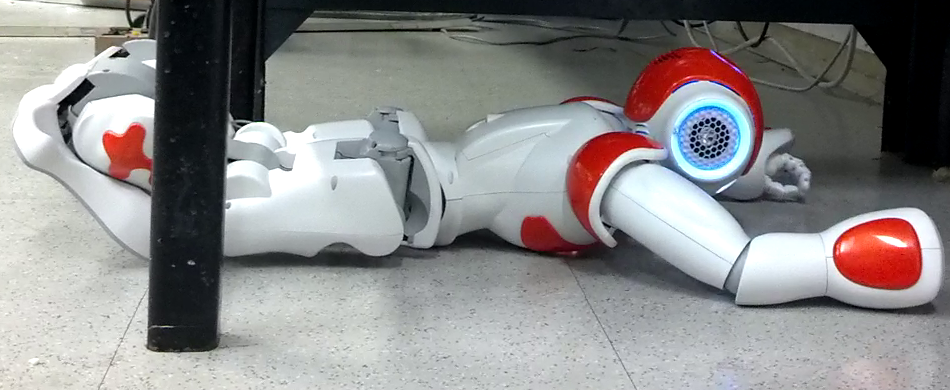
\includegraphics[width=0.33\textwidth]{crawl/under_table/profile_sequence/15.png}

\vspace*{0.05in}
\centering
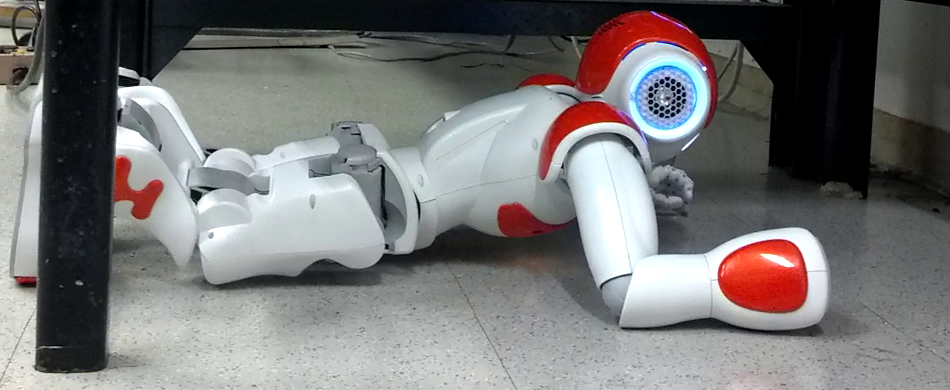
\includegraphics[width=0.33\textwidth]{crawl/under_table/profile_sequence/16.png}
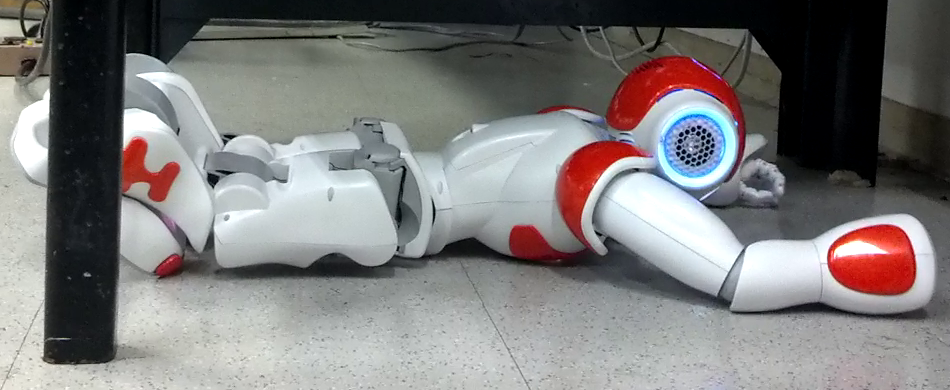
\includegraphics[width=0.33\textwidth]{crawl/under_table/profile_sequence/17.png}
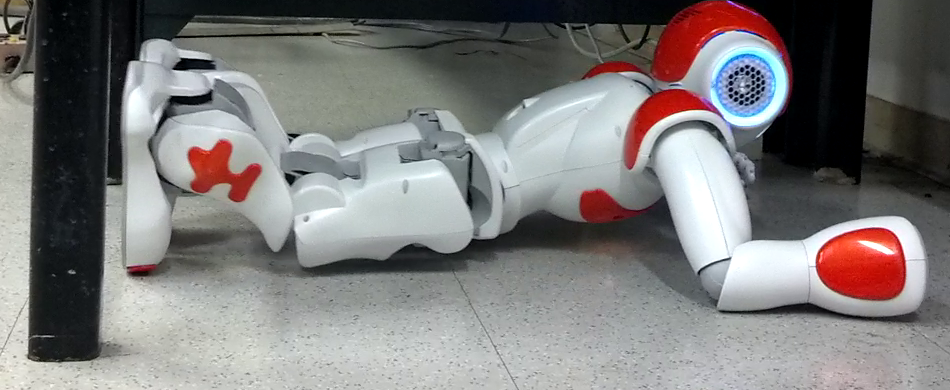
\includegraphics[width=0.33\textwidth]{crawl/under_table/profile_sequence/18.png}

\caption{This figure shows the first experiment of the Nao crawling under the vertically constrained table.}
\label{fig:nao_table_exp1_crawl1}
\end{figure}

% Explain that this experiment is a demonstration of the gait being used to perform a task,
% walking somewhere, getting through a crawl space, and coming out the other side.
Figure~\ref{fig:nao_table_exp2_crawl1}~and~\ref{fig:nao_table_exp2_crawl2} show the second
experiment performed with the vertically constrained table. The robot has detected and walked to
the red marker affixed to the table. It then transitions to a prone posture and begins the crawling
sequence. After having crawled to the other side, the robot transitions to a sitting posture.
The ability to transition from posture to posture is provided through the NAOqi API\@.
For this experiment, the robot executed 25 sequences in 58 seconds. The robot traveled
about 2.75 body lengths or 1,676.4 $mm$, equating to a velocity of 28.9 $\frac{mm}{s}$.

\begin{figure}
    \centerline{
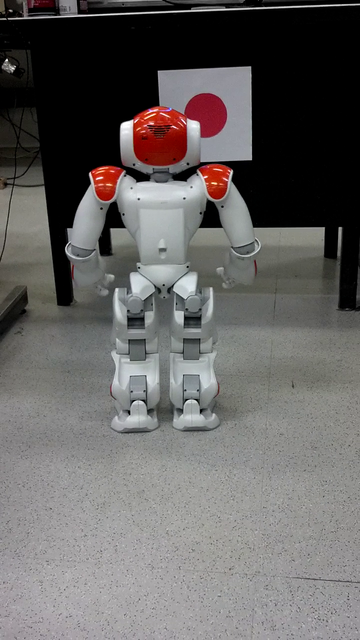
\includegraphics[width=0.2\textwidth]{crawl/walk_to/to/12s.png}
\includegraphics[width=0.2\textwidth]{crawl/walk_to/to/18s.png}
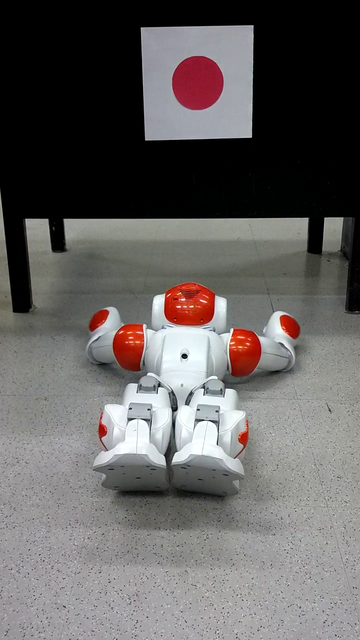
\includegraphics[width=0.2\textwidth]{crawl/walk_to/to/29s.png}
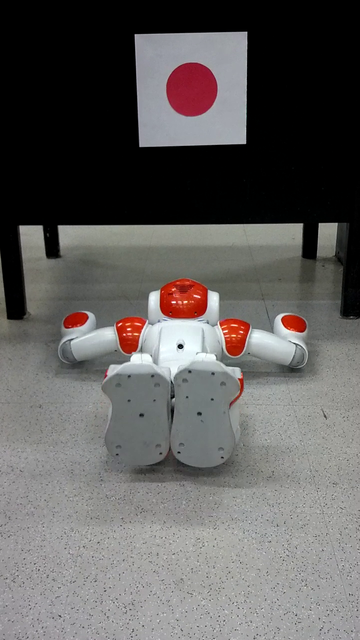
\includegraphics[width=0.2\textwidth]{crawl/walk_to/to/30s_2.png}
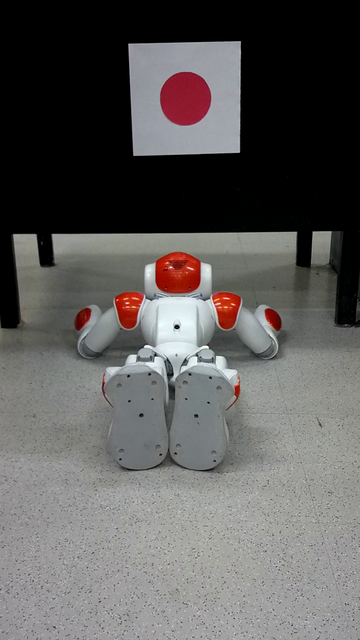
\includegraphics[width=0.2\textwidth]{crawl/walk_to/to/34s.png}
}
\vspace*{0.05in}
\centerline{
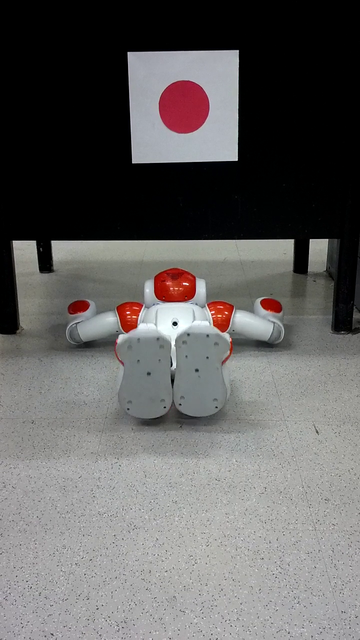
\includegraphics[width=0.2\textwidth]{crawl/walk_to/to/37s.png}
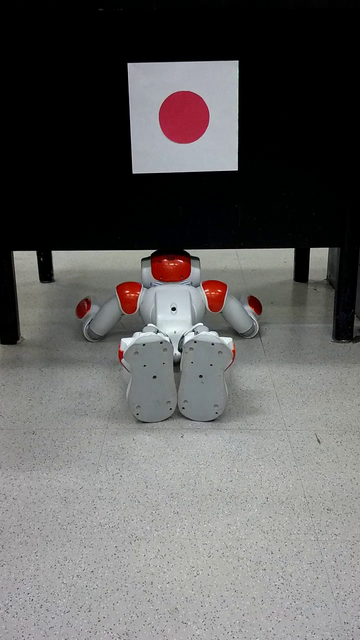
\includegraphics[width=0.2\textwidth]{crawl/walk_to/to/40s.png}
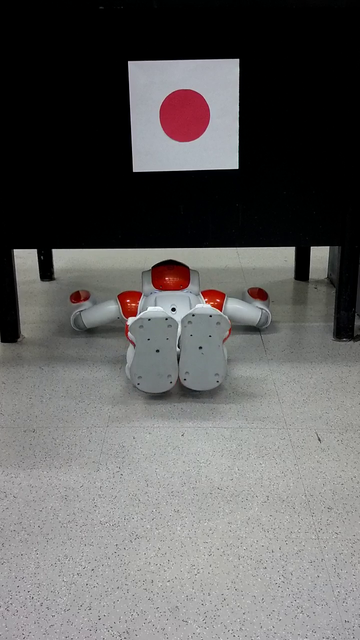
\includegraphics[width=0.2\textwidth]{crawl/walk_to/to/41s.png}
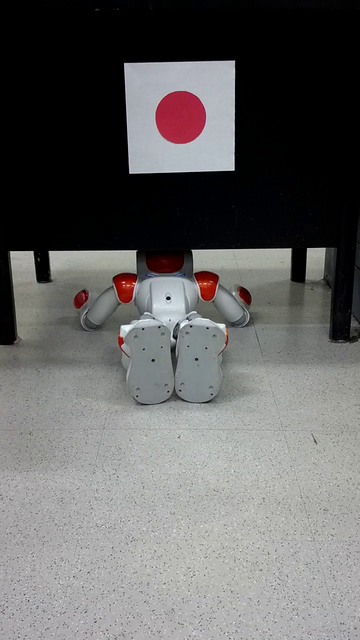
\includegraphics[width=0.2\textwidth]{crawl/walk_to/to/43s.png}
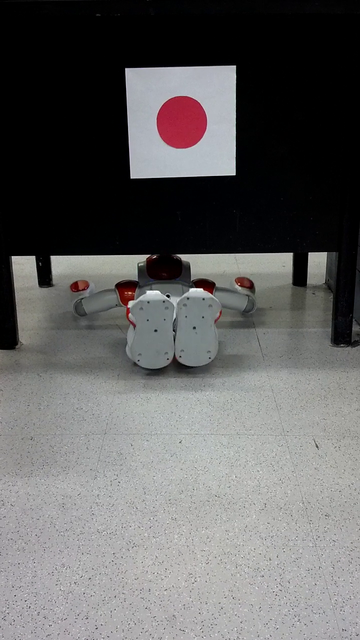
\includegraphics[width=0.2\textwidth]{crawl/walk_to/to/46s.png}
}
\caption{This figure shows the approach portion of the second vertically constrained table experiment.
         A red circle is used as a marker for the direction in which the robot is commanded to move.
         When the robot approaches below a specified distance threshold from the red circle,
         the crouch-down and crawl gait sequence is initiated.}
\label{fig:nao_table_exp2_crawl1}
\end{figure}

\begin{figure}
    \centerline{
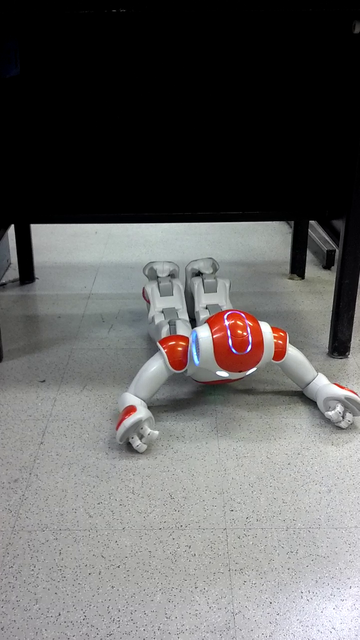
\includegraphics[width=0.2\textwidth]{crawl/walk_to/from/8s.png}
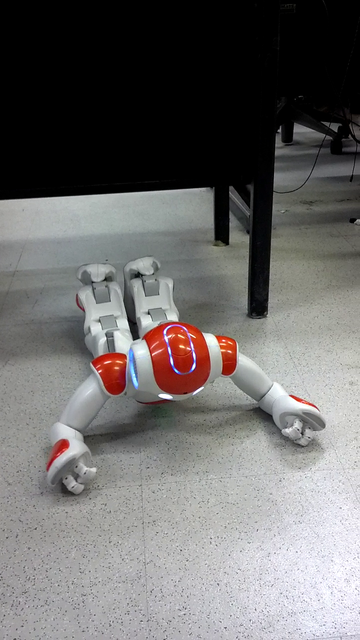
\includegraphics[width=0.2\textwidth]{crawl/walk_to/from/15s.png}
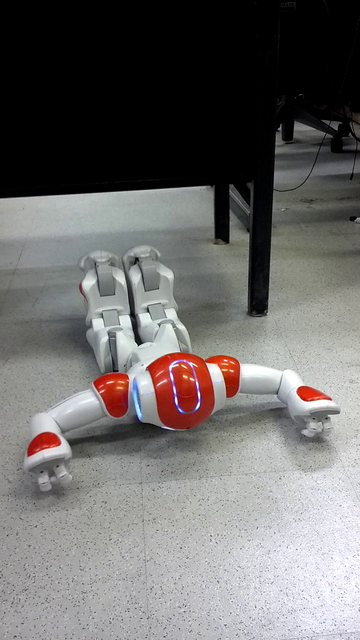
\includegraphics[width=0.2\textwidth]{crawl/walk_to/from/16s.png}
\includegraphics[width=0.2\textwidth]{crawl/walk_to/from/17s.png}
\includegraphics[width=0.2\textwidth]{crawl/walk_to/from/18s.png}
}
\vspace*{0.05in}
\centerline{
\includegraphics[width=0.2\textwidth]{crawl/walk_to/from/24s.png}
\includegraphics[width=0.2\textwidth]{crawl/walk_to/from/30s.png}
\includegraphics[width=0.2\textwidth]{crawl/walk_to/from/32s.png}
\includegraphics[width=0.2\textwidth]{crawl/walk_to/from/35s.png}
\includegraphics[width=0.2\textwidth]{crawl/walk_to/from/37s.png}
}
\caption{This figure shows the recovery portion of the second vertically constrained table experiment.
         After the Nao has executed a set number of crawl sequences, the robot transitions to
         a sitting posture.}
\label{fig:nao_table_exp2_crawl2}
\end{figure}

\subsection{Joint Data} \label{subsec:nom_crawl_joint_data}
The NAOqi API provides functions for recording joint angles and motor currents. During the
nominal crawl gait experiments, these values were recorded and
Figures~\ref{fig:nao_joint_angles1}, \ref{fig:nao_joint_angles_long_seq},
and~\ref{fig:nao_currents} plot the results.
Figure~\ref{fig:nao_joint_angles1} plots the joint angles for the arms and legs of the
robot during the execution of multiple gait cycles. As expected, the plots show a clear
periodicity to the gait.
As the gait is laterally symmetric, the joint angles for the left and right side of the robot
are similar, with the exception of the arm joints below the shoulder pitch.
The joint angle curves for the shoulder roll, elbow yaw, and elbow roll 
shown in Figure~\ref{fig:nao_joint_angles1} have a mirror symmetry rather than being identical.
This is due to the robot frame and joint frame definitions from the NAOqi API\@.
Figure~\ref{fig:nao_arm_joints_reflect1} shows that the joint frame definitions
are such that increasing the shoulder roll angle of each arm rotates each arm to the left.
The elbow yaw and roll joints have a similar behavior. Therefore, to command the arm to
the required positions, the right arm shoulder roll, elbow yaw, and elbow roll angles
are the opposite of the left arm versions.
In addition, the hip-yaw pitch, hip roll, and ankle roll are not symmetric here as they
were set to small constants that do not actively participate in the Projected Profile gait.

\begin{figure}
\centering
\includegraphics[width=0.5\textwidth]{crawl/joint_angles/LeftArmJointAngles.png}
\includegraphics[width=0.5\textwidth]{crawl/joint_angles/LeftLegJointAngles.png}

\centering
\includegraphics[width=0.5\textwidth]{crawl/joint_angles/RightArmJointAngles.png}
\includegraphics[width=0.5\textwidth]{crawl/joint_angles/RightLegJointAngles.png}

\caption{This figure shows the measured joint angles during multiple iterations of the periodic crawling gait.
         The angles for the left and right side can be seen to be identical, except for those
         of the shoulder roll, elbow yaw, and elbow roll. These have a mirror symmetry, due to
         the joint frame definitions.}
\label{fig:nao_joint_angles1}
\end{figure}

Figure~\ref{fig:nao_joint_angles_long_seq} shows the full joint angle sequence as the robot
transitions from standing to crawling. The Nao starts in a standing posture and then transitions
to a crouch posture. From there, it transitions to the initial crawling pose and begins to
crawl. It executes five crawl sequences to simulate crawling under an object.
Only five sequences were performed in order to make the plot of the joint angles easier to present.
The robot then transitions back to the crouching posture. Each of the posture transitions was
executed using the NAOqi ALRobotPosture API\@.
Figure~\ref{fig:nao_postures1} shows the different postures used in these transitions.

\begin{figure}
\centering
\includegraphics[width=0.5\textwidth]{crawl/joint_angles_long_sequence/LeftArmJointAngles_longSequence.png}
\includegraphics[width=0.5\textwidth]{crawl/joint_angles_long_sequence/LeftLegJointAngles_longSequence.png}

\centering
\includegraphics[width=0.5\textwidth]{crawl/joint_angles_long_sequence/RightArmJointAngles_longSequence.png}
\includegraphics[width=0.5\textwidth]{crawl/joint_angles_long_sequence/RightLegJointAngles_longSequence.png}

\caption{Measured joint angles for a sequence of transitioning from standing to crouch to crawling,
         crawling under a table, and then returning to crouch.}
\label{fig:nao_joint_angles_long_seq}
\end{figure}

% This plot shows the current draws of the arm and leg joints.
% There are some distinct patterns, but is hard to relate torques directly.
While the Nao platform is equipped with encoders that can directly measure joint
angle, it is not equipped with joint torque sensors. The robot is equipped with sensors
that measure joint motor current which can be used to estimate joint torque. The motor currents
were recorded for several crawl sequences and are presented in Figure~\ref{fig:nao_currents}.
While the plots do show a periodicity to the motor current draws, it is difficult to observe
other useful information. Though there is a relationship between motor current and joint torque, 
in general, current sensors give a poor estimate of torque. One limiting factor is that each joint uses
some form of motor control to bring the joint to a desired angle. This controller will
obfuscate the torque-current relationship as it draws power to position the joint.
Therefore, the joint current plots are of limited use.

\begin{figure}
\centering
\includegraphics[width=0.5\textwidth]{crawl/current_draws/LeftArmCurrentDraw.png}
\includegraphics[width=0.5\textwidth]{crawl/current_draws/LeftLegCurrentDraw.png}

\caption{Measured motor current draws during multiple iterations of the periodic crawling gait.}
\label{fig:nao_currents}
\end{figure}




\FloatBarrier
\section{Optimized Crawl Gait Data} \label{sec:opt_crawl_data}

To test the Projected Profile gait using the optimal parameters reviewed in 
Section~\ref{subsec:gait_params}, the gait sequence was generated in
MATLAB and simulated in V-REP\@. The closed chain phase of the gait was the
only portion that was optimized, so this phase of the gait was simulated and
analyzed. As reviewed in Section~\ref{subsec:crawl_environments}, the V-REP simulator
provides joint torque simulation and sensing, which can be recorded to evaluate
the increase in gait efficiency using these parameters.

\subsection{Simulations}

% Here's the MATLAB simulation. The theta 3 and 4 are doing different things.
Figure~\ref{fig:pp_opt_gait1} shows samples of the simplified kinematic model,
as it executes the closed chain phase of the optimized Projected Profile gait.
As with the nominal crawl gait, the angle $\alpha$ transitions from $-30^\circ$ to $-90^\circ$,
though not linearly, as reviewed in Section~\ref{subsec:gait_params}.
While it is difficult to see the difference in the optimized $\alpha$ trajectory from the
nominal version, the trajectory of $\theta_3$ and $\theta_4$ are quite different
from those seen in Figure~\ref{fig:pp_nom_gait1}. As opposed to the nominal gait
which appears to hold the midsection of the model low to the ground, the optimized
gait arches the midsection upwards as the gait progresses, before being brought down. This resembles the tendency for humans to arch their back when attempting
to support their weight in similar positions.

\begin{figure}
\centering
\includegraphics[width=0.5\textwidth]{crawl/pp/optimal/angle30_1.png}
\includegraphics[width=0.5\textwidth]{crawl/pp/optimal/angle42.7474_1.png}

\centering
\includegraphics[width=0.5\textwidth]{crawl/pp/optimal/angle54.5496_1.png}
\includegraphics[width=0.5\textwidth]{crawl/pp/optimal/angle66.4421_1.png}

\centering
\includegraphics[width=0.5\textwidth]{crawl/pp/optimal/angle78.1161_1.png}
\includegraphics[width=0.5\textwidth]{crawl/pp/optimal/angle89.9428_1.png}

\caption{This figure shows the simplified kinematic model executing the close
         chain phase of the optimized gait.}
\label{fig:pp_opt_gait1}
\end{figure}

% Here's the V-REP simulation. The knees and hips are doing different things.
% The arms are down the whole time.
The V-REP simulation of the Nao executing the optimized gait can be seen in
Figure~\ref{fig:vrep_nao_opt_gait1}. As with the
simplified kinematic model, the Nao can be seen to be using its hips and knees to arch its back during the gait sequence.

\begin{figure}
\centering
\includegraphics[width=0.5\textwidth]{crawl/vrep/optimized/1.png}
\includegraphics[width=0.5\textwidth]{crawl/vrep/optimized/2.png}

\centering
\includegraphics[width=0.5\textwidth]{crawl/vrep/optimized/3.png}
\includegraphics[width=0.5\textwidth]{crawl/vrep/optimized/4.png}

\centering
\includegraphics[width=0.5\textwidth]{crawl/vrep/optimized/5.png}

\caption{This figure shows the simulated Nao executing the closed chain phase of the
         optimized gait.}
\label{fig:vrep_nao_opt_gait1}
\end{figure}

\subsection{Joint Torque Data} \label{subsec:opt_joint_torque_data}

% Ok, so now, how does it do with these new optimizations?
% We use the V-REP here instead of the currents from the robot because they are easier to interpret.
In order to analyze the efficiency increase to the gait using the optimal gait parameters,
the torques from the simulated Nao were recorded during nominal and optimal closed chain
phase gait executions. The simulated torques are easier to interpret than the motor currents
presented in Section~\ref{subsec:nom_crawl_joint_data} as they directly represent the torques
the Nao would experience during a crawl. The ankle pitch, knee pitch, hip pitch, and shoulder pitch
torques of the simulated Nao were recorded, corresponding to the Projected Profile joints 
$[\theta_2, \theta_3, \theta_4, \theta_5]$. These were the joints which were used in the optimization
procedure and were therefore recorded for analysis.
To test the efficacy of the pseudo-static assumption, the crawl gaits were executed at different
speeds so that the effects of transient torques would be present to varying degrees.
As discussed in Chapter~\ref{subsec:crawl_pseudo_static_model}, the pseudo-static
model assumes that gravity is the dominant force in the system and the  transients
do not affect the system significantly.
Ten speeds were tested for each gait. The duration of each closed chain gait phase varied from one second to
ten seconds, in one second increments. The transient torques will have a stronger influence
on the joint torques at the higher speeds.

% Here are the torques, one after another.
% They seem to look similar after a certain point. This is cycle invariance, where the 
% pseudo static model wins.
% In the beginning though, they look as if they're being compressed. You can see
% there is a time invariant part. This is where the dynamics hold sway. After
% this point, they diverge.
Figures~\ref{fig:vrep_nom_joint_torques_by_duration1}~and~\ref{fig:vrep_opt_joint_torques_by_duration1}
show joint torque plots from the nominal and optimal gaits, respectively.
Each panel shows the torques for each of the four joints, over the prescribed gait duration.
Only a subset of the experiments are shown as the differences between panels diminishes
as the duration increases. This is likely due to a shift from the dominant component 
of the system being the transient torques to the pseudo-statics.

\begin{figure}
\centering
\includegraphics[width=0.5\textwidth]{crawl/torques/nom_torques_duration_1.0_1.png}
\includegraphics[width=0.5\textwidth]{crawl/torques/nom_torques_duration_2.0_1.png}

\centering
\includegraphics[width=0.5\textwidth]{crawl/torques/nom_torques_duration_3.0_1.png}
\includegraphics[width=0.5\textwidth]{crawl/torques/nom_torques_duration_5.0_1.png}

\centering
\includegraphics[width=0.5\textwidth]{crawl/torques/nom_torques_duration_7.0_1.png}
\includegraphics[width=0.5\textwidth]{crawl/torques/nom_torques_duration_10.0_1.png}

\caption{This figure shows the nominal joint torque curves for six durations.
         As the duration increased, the graphs show less variation.}
\label{fig:vrep_nom_joint_torques_by_duration1}
\end{figure}

\begin{figure}
\centering
\includegraphics[width=0.5\textwidth]{crawl/torques/opt_torques_duration_1.0_1.png}
\includegraphics[width=0.5\textwidth]{crawl/torques/opt_torques_duration_2.0_1.png}

\centering
\includegraphics[width=0.5\textwidth]{crawl/torques/opt_torques_duration_3.0_1.png}
\includegraphics[width=0.5\textwidth]{crawl/torques/opt_torques_duration_5.0_1.png}

\centering
\includegraphics[width=0.5\textwidth]{crawl/torques/opt_torques_duration_7.0_1.png}
\includegraphics[width=0.5\textwidth]{crawl/torques/opt_torques_duration_10.0_1.png}

\caption{This figure shows the optimal joint torque curves for six durations.
         As the duration increased, the graphs show less variation.}
\label{fig:vrep_opt_joint_torques_by_duration1}
\end{figure}

Figures~\ref{fig:vrep_nom_joint_torques_by_joint_over_time1}~and~\ref{fig:vrep_opt_joint_torques_by_joint_over_time1}
show the torque curves for each joint as a function of time.
The panels overlay the torques onto each other
which shows their similarity during the initial portion of the gait, before fanning out
in the later portion.
This similarity is demonstrated more clearly in Figures~\ref{fig:vrep_nom_joint_transient_torques_by_joint1}
and~\ref{fig:vrep_opt_joint_transient_torques_by_joint1}, which highlight the transients.
For the nominal gait, the joint torque curves for each joint from about $t = 0.0$ seconds to $t = 0.25$ seconds
are similar regardless of the gait duration. The optimal gait has a similar time interval
at around $t = 0.0$ seconds to $t = 0.175$ seconds. After these points, as seen in
Figures~\ref{fig:vrep_nom_joint_torques_by_joint_over_time1}~and~\ref{fig:vrep_opt_joint_torques_by_joint_over_time1},
the curves tend to diverge.
This gait-duration-invariant-with-respect-to-time portion suggests that the system transients are the dominant
forces in this region. For the shorter duration gaits, this means the transients dominate as much as
20\% of the gait cycle. But as the gait cycle duration is increased, the transients
contribute to a diminishing percentage of the gait cycle, which appears as the left most
portion of the panels in Figures~\ref{fig:vrep_nom_joint_torques_by_duration1}~and~\ref{fig:vrep_opt_joint_torques_by_duration1}
being compressed. 
The differences between the 7 and 10 second gaits for example,
are less pronounced than between the 1 and 3 second gaits.

\begin{figure}
\centering
\includegraphics[width=0.5\textwidth]{crawl/torques/trimmed/nom_joint2_time_torques.png}
\includegraphics[width=0.5\textwidth]{crawl/torques/trimmed/nom_joint3_time_torques.png}

\centering
\includegraphics[width=0.5\textwidth]{crawl/torques/trimmed/nom_joint4_time_torques.png}
\includegraphics[width=0.5\textwidth]{crawl/torques/trimmed/nom_joint5_time_torques.png}

\caption{This figure shows the nominal joint torque curves as a function of time.
         Each panel shows the curves for one joint. The curves can be seen to be similar
         up to a certain time, at which point they diverge. 
         Figure~\ref{fig:vrep_nom_joint_transient_torques_by_joint1} shows a magnified
         view of the similar portions of the curves.}
\label{fig:vrep_nom_joint_torques_by_joint_over_time1}
\end{figure}

\begin{figure}
\centering
\includegraphics[width=0.5\textwidth]{crawl/torques/trimmed/opt_joint2_time_torques.png}
\includegraphics[width=0.5\textwidth]{crawl/torques/trimmed/opt_joint3_time_torques.png}

\centering
\includegraphics[width=0.5\textwidth]{crawl/torques/trimmed/opt_joint4_time_torques.png}
\includegraphics[width=0.5\textwidth]{crawl/torques/trimmed/opt_joint5_time_torques.png}

\caption{This figure shows the optimal joint torque curves as a function of time.
         Each panel shows the curves for one joint. The curves can be seen to be similar
         up to a certain time, at which point they diverge.
         Figure~\ref{fig:vrep_opt_joint_transient_torques_by_joint1} shows a magnified
         view of the similar portions of the curves.}
\label{fig:vrep_opt_joint_torques_by_joint_over_time1}
\end{figure}

\begin{figure}
\centering
\includegraphics[width=0.5\textwidth]{crawl/torques/trimmed/nom_joint2_trans_torques.png}
\includegraphics[width=0.5\textwidth]{crawl/torques/trimmed/nom_joint3_trans_torques.png}

\centering
\includegraphics[width=0.5\textwidth]{crawl/torques/trimmed/nom_joint4_trans_torques.png}
\includegraphics[width=0.5\textwidth]{crawl/torques/trimmed/nom_joint5_trans_torques.png}

\caption{This figure shows a magnified view of the nominal joint torque curves as a function of time.
         Each panel shows the curves for one joint. The curves are overlaid to show their
         similarities when viewed with respect to time. The dashed black line signifies
         the time at which the curves diverge.}
\label{fig:vrep_nom_joint_transient_torques_by_joint1}
\end{figure}

\begin{figure}
\centering
\includegraphics[width=0.5\textwidth]{crawl/torques/trimmed/opt_joint2_trans_torques.png}
\includegraphics[width=0.5\textwidth]{crawl/torques/trimmed/opt_joint3_trans_torques.png}

\centering
\includegraphics[width=0.5\textwidth]{crawl/torques/trimmed/opt_joint4_trans_torques.png}
\includegraphics[width=0.5\textwidth]{crawl/torques/trimmed/opt_joint5_trans_torques.png}

\caption{This figure shows a magnified view of the optimal joint torque curves as a function of time.
         Each panel shows the curves for one joint. The curves are overlaid to show their
         similarities when viewed with respect to time. The dashed black line signifies
         the time at which the curves diverge.}
\label{fig:vrep_opt_joint_transient_torques_by_joint1}
\end{figure}

This similarity is more clearly demonstrated in
Figures~\ref{fig:vrep_nom_joint_torques_by_joint_over_cycle1}~and~\ref{fig:vrep_opt_joint_torques_by_joint_over_cycle1}.
These panels plot joint torques
for each joint as a function of gait cycle percentage, rather than time. Within each of the
panels, the joint torques from 20\% to 100\% can be seen to be similar between durations. 
This gait-duration-invariant-with-respect-to-cycle-percentage portion suggests that
the pseudo-statics are the dominant forces in this region. This is because joint torques
are now only a function of position and not the time it takes to get to that position.

\begin{figure}
\centering
\includegraphics[width=0.5\textwidth]{crawl/torques/trimmed/nom_joint2_torques.png}
\includegraphics[width=0.5\textwidth]{crawl/torques/trimmed/nom_joint3_torques.png}

\centering
\includegraphics[width=0.5\textwidth]{crawl/torques/trimmed/nom_joint4_torques.png}
\includegraphics[width=0.5\textwidth]{crawl/torques/trimmed/nom_joint5_torques.png}

\caption{This figure shows the nominal joint torque curves as a function of gait cycle percentage.
         Each panel shows the curves for one joint. The curves are overlaid to show their
         similarities when viewed with respect to cycle percentage.}
\label{fig:vrep_nom_joint_torques_by_joint_over_cycle1}
\end{figure}

\begin{figure}
\centering
\includegraphics[width=0.5\textwidth]{crawl/torques/trimmed/opt_joint2_torques.png}
\includegraphics[width=0.5\textwidth]{crawl/torques/trimmed/opt_joint3_torques.png}

\centering
\includegraphics[width=0.5\textwidth]{crawl/torques/trimmed/opt_joint4_torques.png}
\includegraphics[width=0.5\textwidth]{crawl/torques/trimmed/opt_joint5_torques.png}

\caption{This figure shows the optimal joint torque curves as a function of gait cycle percentage.
         Each panel shows the curves for one joint. The curves are overlaid to show their
         similarities when viewed with respect to cycle percentage.}
\label{fig:vrep_opt_joint_torques_by_joint_over_cycle1}
\end{figure}

% Side by side it looks like the optimal one has shifted the affine region to the left.
% So for short durations when the dynamics win, the optimized one and the nominal one
% are different, but there's no clear pattern, though there are some reduced amplitudes.
% For the longer ones, the optimal one seems to compress what might look like transients,
% and hold everything at the shallower slopes longer.
When comparing the nominal gait torque curves to the optimal ones, as in
Figure~\ref{fig:vrep_comparison_joint_torques_by_duration1}, a number of effects can be seen.
For short duration gaits where the transient dynamics are dominant, a pattern is less
obvious though the amplitude of the torque transients for joints $\theta_3$ and $\theta_4$
have been reduced. In the Nao, these are the knee pitch and hip pitch joints.
In the longer duration gaits, the optimization appears to have the effect of compressing
the transients to the left and reaching the affine region of the torque curve more quickly.
This means while the torque curves do transit through these higher magnitude regions,
they spend less time there and therefore accrue a lower torque cost.

\begin{figure}
\centering
\includegraphics[width=0.5\textwidth]{crawl/torques/nom_torques_duration_1.0_1.png}
\includegraphics[width=0.5\textwidth]{crawl/torques/opt_torques_duration_1.0_1.png}

\centering
\includegraphics[width=0.5\textwidth]{crawl/torques/nom_torques_duration_5.0_1.png}
\includegraphics[width=0.5\textwidth]{crawl/torques/opt_torques_duration_5.0_1.png}

\centering
\includegraphics[width=0.5\textwidth]{crawl/torques/nom_torques_duration_10.0_1.png}
\includegraphics[width=0.5\textwidth]{crawl/torques/opt_torques_duration_10.0_1.png}

\caption{This figure compares the joint torque curves of the nominal and optimal
         gaits for three gait durations. The optimal curves extend the affine portion to the left, 
         reducing the transient response.}
\label{fig:vrep_comparison_joint_torques_by_duration1}
\end{figure}


% Actually summing up the costs you can see there's a difference between the two and the optimal
% one is always lower cost.
% Percentagewise, the 7 second gait had the biggest difference, but I'd say that anything after
% 7 seconds has probably converges and takes the most advantage of the optimization.
% These costs are for straight sum of torques. They're not weighted.
Examining the torque costs of the two gaits as a function of duration
in Figure~\ref{fig:cost_duration1} supports
the idea that as the effects of the transients diminishes and the pseudo-statics
become more dominant, the efficacy of the optimization increases.
This is expected as the optimization was formulated with this assumption. 
It should be noted that the costs presented in Figure~\ref{fig:cost_duration1}
are not weighted according to the weight vector presented in Chapter~\ref{subsec:cost_functions}.
The figure shows the integral of the costs with the weight vector $w = [1, 1, 1, 1]^T$
in order to show the simple torque cost to the robot. 
The absolute and percentage difference in costs for the short durations is small,
though the optimal gait always outperforms the nominal gait.
As the duration increases, the optimal gait costs up to 21.5\% less than the
nominal gait. Therefore, while the optimal gait does not always outperform the
nominal gait by a significant amount, it is always preferable to the nominal gait.

\begin{figure}
\includegraphics[width=0.5\textwidth]{crawl/cost/gait_cost_duration1.png}
\includegraphics[width=0.5\textwidth]{crawl/cost/cost_imp_duration1.png}
\caption{This figure shows cost comparisons between the optimal and
         nominal gaits as a function of gait duration. The left panel shows
         this in terms of absolute cost and the right panel shows this in 
         terms of percentage. The right panel percentage is the ratio $\frac{C_o}{C_n}$
         for each duration, where $C_o$ is the optimal gait cost, and $C_n$ is the nominal gait cost.}
\label{fig:cost_duration1}
\end{figure}
